%********************************************%
%*       Generated from PreTeXt source      *%
%*       on 2021-04-26T12:28:30-03:00       *%
%*   A recent stable commit (2020-08-09):   *%
%* 98f21740783f166a773df4dc83cab5293ab63a4a *%
%*                                          *%
%*         https://pretextbook.org          *%
%*                                          *%
%********************************************%
%% We elect to always write snapshot output into <job>.dep file
\RequirePackage{snapshot}
\documentclass[oneside,10pt,]{article}
%% Custom Preamble Entries, early (use latex.preamble.early)
%% Default LaTeX packages
%%   1.  always employed (or nearly so) for some purpose, or
%%   2.  a stylewriter may assume their presence
\usepackage{geometry}
%% Some aspects of the preamble are conditional,
%% the LaTeX engine is one such determinant
\usepackage{ifthen}
%% etoolbox has a variety of modern conveniences
\usepackage{etoolbox}
\usepackage{ifxetex,ifluatex}
%% Raster graphics inclusion
\usepackage{graphicx}
%% Color support, xcolor package
%% Always loaded, for: add/delete text, author tools
%% Here, since tcolorbox loads tikz, and tikz loads xcolor
\PassOptionsToPackage{usenames,dvipsnames,svgnames,table}{xcolor}
\usepackage{xcolor}
%% begin: defined colors, via xcolor package, for styling
%% end: defined colors, via xcolor package, for styling
%% Colored boxes, and much more, though mostly styling
%% skins library provides "enhanced" skin, employing tikzpicture
%% boxes may be configured as "breakable" or "unbreakable"
%% "raster" controls grids of boxes, aka side-by-side
\usepackage{tcolorbox}
\tcbuselibrary{skins}
\tcbuselibrary{breakable}
\tcbuselibrary{raster}
%% We load some "stock" tcolorbox styles that we use a lot
%% Placement here is provisional, there will be some color work also
%% First, black on white, no border, transparent, but no assumption about titles
\tcbset{ bwminimalstyle/.style={size=minimal, boxrule=-0.3pt, frame empty,
colback=white, colbacktitle=white, coltitle=black, opacityfill=0.0} }
%% Second, bold title, run-in to text/paragraph/heading
%% Space afterwards will be controlled by environment,
%% independent of constructions of the tcb title
%% Places \blocktitlefont onto many block titles
\tcbset{ runintitlestyle/.style={fonttitle=\blocktitlefont\upshape\bfseries, attach title to upper} }
%% Spacing prior to each exercise, anywhere
\tcbset{ exercisespacingstyle/.style={before skip={1.5ex plus 0.5ex}} }
%% Spacing prior to each block
\tcbset{ blockspacingstyle/.style={before skip={2.0ex plus 0.5ex}} }
%% xparse allows the construction of more robust commands,
%% this is a necessity for isolating styling and behavior
%% The tcolorbox library of the same name loads the base library
\tcbuselibrary{xparse}
%% Hyperref should be here, but likes to be loaded late
%%
%% Inline math delimiters, \(, \), need to be robust
%% 2016-01-31:  latexrelease.sty  supersedes  fixltx2e.sty
%% If  latexrelease.sty  exists, bugfix is in kernel
%% If not, bugfix is in  fixltx2e.sty
%% See:  https://tug.org/TUGboat/tb36-3/tb114ltnews22.pdf
%% and read "Fewer fragile commands" in distribution's  latexchanges.pdf
\IfFileExists{latexrelease.sty}{}{\usepackage{fixltx2e}}
%% shorter subnumbers in some side-by-side require manipulations
\usepackage{xstring}
%% Text height identically 9 inches, text width varies on point size
%% See Bringhurst 2.1.1 on measure for recommendations
%% 75 characters per line (count spaces, punctuation) is target
%% which is the upper limit of Bringhurst's recommendations
\geometry{letterpaper,total={340pt,9.0in}}
%% Custom Page Layout Adjustments (use latex.geometry)
%% This LaTeX file may be compiled with pdflatex, xelatex, or lualatex executables
%% LuaTeX is not explicitly supported, but we do accept additions from knowledgeable users
%% The conditional below provides  pdflatex  specific configuration last
%% begin: engine-specific capabilities
\ifthenelse{\boolean{xetex} \or \boolean{luatex}}{%
%% begin: xelatex and lualatex-specific default configuration
\ifxetex\usepackage{xltxtra}\fi
%% realscripts is the only part of xltxtra relevant to lualatex 
\ifluatex\usepackage{realscripts}\fi
%% end:   xelatex and lualatex-specific default configuration
}{
%% begin: pdflatex-specific default configuration
%% We assume a PreTeXt XML source file may have Unicode characters
%% and so we ask LaTeX to parse a UTF-8 encoded file
%% This may work well for accented characters in Western language,
%% but not with Greek, Asian languages, etc.
%% When this is not good enough, switch to the  xelatex  engine
%% where Unicode is better supported (encouraged, even)
\usepackage[utf8]{inputenc}
%% end: pdflatex-specific default configuration
}
%% end:   engine-specific capabilities
%%
%% Fonts.  Conditional on LaTex engine employed.
%% Default Text Font: The Latin Modern fonts are
%% "enhanced versions of the [original TeX] Computer Modern fonts."
%% We use them as the default text font for PreTeXt output.
%% Default Monospace font: Inconsolata (aka zi4)
%% Sponsored by TUG: http://levien.com/type/myfonts/inconsolata.html
%% Loaded for documents with intentional objects requiring monospace
%% See package documentation for excellent instructions
%% fontspec will work universally if we use filename to locate OTF files
%% Loads the "upquote" package as needed, so we don't have to
%% Upright quotes might come from the  textcomp  package, which we also use
%% We employ the shapely \ell to match Google Font version
%% pdflatex: "varl" package option produces shapely \ell
%% pdflatex: "var0" package option produces plain zero (not used)
%% pdflatex: "varqu" package option produces best upright quotes
%% xelatex,lualatex: add OTF StylisticSet 1 for shapely \ell
%% xelatex,lualatex: add OTF StylisticSet 2 for plain zero (not used)
%% xelatex,lualatex: add OTF StylisticSet 3 for upright quotes
%%
%% Automatic Font Control
%% Portions of a document, are, or may, be affected by defined commands
%% These are perhaps more flexible when using  xelatex  rather than  pdflatex
%% The following definitions are meant to be re-defined in a style, using \renewcommand
%% They are scoped when employed (in a TeX group), and so should not be defined with an argument
\newcommand{\divisionfont}{\relax}
\newcommand{\blocktitlefont}{\relax}
\newcommand{\contentsfont}{\relax}
\newcommand{\pagefont}{\relax}
\newcommand{\tabularfont}{\relax}
\newcommand{\xreffont}{\relax}
\newcommand{\titlepagefont}{\relax}
%%
\ifthenelse{\boolean{xetex} \or \boolean{luatex}}{%
%% begin: font setup and configuration for use with xelatex
%% Generally, xelatex is necessary for non-Western fonts
%% fontspec package provides extensive control of system fonts,
%% meaning *.otf (OpenType), and apparently *.ttf (TrueType)
%% that live *outside* your TeX/MF tree, and are controlled by your *system*
%% (it is possible that a TeX distribution will place fonts in a system location)
%%
%% The fontspec package is the best vehicle for using different fonts in  xelatex
%% So we load it always, no matter what a publisher or style might want
%%
\usepackage{fontspec}
%%
%% begin: xelatex main font ("font-xelatex-main" template)
%% Latin Modern Roman is the default font for xelatex and so is loaded with a TU encoding
%% *in the format* so we can't touch it, only perhaps adjust it later
%% in one of two ways (then known by NFSS names such as "lmr")
%% (1) via NFSS with font family names such as "lmr" and "lmss"
%% (2) via fontspec with commands like \setmainfont{Latin Modern Roman}
%% The latter requires the font to be known at the system-level by its font name,
%% but will give access to OTF font features through optional arguments
%% https://tex.stackexchange.com/questions/470008/
%% where-and-how-does-fontspec-sty-specify-the-default-font-latin-modern-roman
%% http://tex.stackexchange.com/questions/115321
%% /how-to-optimize-latin-modern-font-with-xelatex
%%
%% end:   xelatex main font ("font-xelatex-main" template)
%% begin: xelatex mono font ("font-xelatex-mono" template)
%% (conditional on non-trivial uses being present in source)
\IfFontExistsTF{Inconsolatazi4-Regular.otf}{}{\GenericError{}{The font "Inconsolatazi4-Regular.otf" requested by PreTeXt output is not available.  Either a file cannot be located in default locations via a filename, or a font is not known by its name as part of your system.}{Consult the PreTeXt Guide for help with LaTeX fonts.}{}}
\IfFontExistsTF{Inconsolatazi4-Bold.otf}{}{\GenericError{}{The font "Inconsolatazi4-Bold.otf" requested by PreTeXt output is not available.  Either a file cannot be located in default locations via a filename, or a font is not known by its name as part of your system.}{Consult the PreTeXt Guide for help with LaTeX fonts.}{}}
\usepackage{zi4}
\setmonofont[BoldFont=Inconsolatazi4-Bold.otf,StylisticSet={1,3}]{Inconsolatazi4-Regular.otf}
%% end:   xelatex mono font ("font-xelatex-mono" template)
%% begin: xelatex font adjustments ("font-xelatex-style" template)
%% end:   xelatex font adjustments ("font-xelatex-style" template)
%%
%% Extensive support for other languages
\usepackage{polyglossia}
%% Set main/default language based on pretext/@xml:lang value
%% Enable secondary languages based on discovery of @xml:lang values
%% Enable fonts/scripts based on discovery of @xml:lang values
%% Western languages should be ably covered by Latin Modern Roman
%% end:   font setup and configuration for use with xelatex
}{%
%% begin: font setup and configuration for use with pdflatex
%% begin: pdflatex main font ("font-pdflatex-main" template)
\usepackage{lmodern}
\usepackage[T1]{fontenc}
%% end:   pdflatex main font ("font-pdflatex-main" template)
%% begin: pdflatex mono font ("font-pdflatex-mono" template)
%% (conditional on non-trivial uses being present in source)
\usepackage[varqu,varl]{inconsolata}
%% end:   pdflatex mono font ("font-pdflatex-mono" template)
%% begin: pdflatex font adjustments ("font-pdflatex-style" template)
%% end:   pdflatex font adjustments ("font-pdflatex-style" template)
%% end:   font setup and configuration for use with pdflatex
}
%% Micromanage spacing, etc.  The named "microtype-options"
%% template may be employed to fine-tune package behavior
\usepackage{microtype}
%% Symbols, align environment, commutative diagrams, bracket-matrix
\usepackage{amsmath}
\usepackage{amscd}
\usepackage{amssymb}
%% allow page breaks within display mathematics anywhere
%% level 4 is maximally permissive
%% this is exactly the opposite of AMSmath package philosophy
%% there are per-display, and per-equation options to control this
%% split, aligned, gathered, and alignedat are not affected
\allowdisplaybreaks[4]
%% allow more columns to a matrix
%% can make this even bigger by overriding with  latex.preamble.late  processing option
\setcounter{MaxMatrixCols}{30}
%%
%%
%% Division Titles, and Page Headers/Footers
%% titlesec package, loading "titleps" package cooperatively
%% See code comments about the necessity and purpose of "explicit" option.
%% The "newparttoc" option causes a consistent entry for parts in the ToC 
%% file, but it is only effective if there is a \titleformat for \part.
%% "pagestyles" loads the  titleps  package cooperatively.
\usepackage[explicit, newparttoc, pagestyles]{titlesec}
%% The companion titletoc package for the ToC.
\usepackage{titletoc}
%% begin: customizations of page styles via the modal "titleps-style" template
%% Designed to use commands from the LaTeX "titleps" package
\pagestyle{plain}
%% end: customizations of page styles via the modal "titleps-style" template
%%
%% Create globally-available macros to be provided for style writers
%% These are redefined for each occurence of each division
\newcommand{\divisionnameptx}{\relax}%
\newcommand{\titleptx}{\relax}%
\newcommand{\subtitleptx}{\relax}%
\newcommand{\shortitleptx}{\relax}%
\newcommand{\authorsptx}{\relax}%
\newcommand{\epigraphptx}{\relax}%
%% Create environments for possible occurences of each division
%% Environment for a PTX "section" at the level of a LaTeX "section"
\NewDocumentEnvironment{sectionptx}{mmmmmm}
{%
\renewcommand{\divisionnameptx}{Seção}%
\renewcommand{\titleptx}{#1}%
\renewcommand{\subtitleptx}{#2}%
\renewcommand{\shortitleptx}{#3}%
\renewcommand{\authorsptx}{#4}%
\renewcommand{\epigraphptx}{#5}%
\section[{#3}]{#1}%
\label{#6}%
}{}%
%% Environment for a PTX "subsection" at the level of a LaTeX "subsection"
\NewDocumentEnvironment{subsectionptx}{mmmmmm}
{%
\renewcommand{\divisionnameptx}{Subseção}%
\renewcommand{\titleptx}{#1}%
\renewcommand{\subtitleptx}{#2}%
\renewcommand{\shortitleptx}{#3}%
\renewcommand{\authorsptx}{#4}%
\renewcommand{\epigraphptx}{#5}%
\subsection[{#3}]{#1}%
\label{#6}%
}{}%
%% Environment for a PTX "exercises" at the level of a LaTeX "subsection"
\NewDocumentEnvironment{exercises-subsection}{mmmmmm}
{%
\renewcommand{\divisionnameptx}{Exercícios}%
\renewcommand{\titleptx}{#1}%
\renewcommand{\subtitleptx}{#2}%
\renewcommand{\shortitleptx}{#3}%
\renewcommand{\authorsptx}{#4}%
\renewcommand{\epigraphptx}{#5}%
\subsection[{#3}]{#1}%
\label{#6}%
}{}%
%% Environment for a PTX "exercises" at the level of a LaTeX "subsection"
\NewDocumentEnvironment{exercises-subsection-numberless}{mmmmmm}
{%
\renewcommand{\divisionnameptx}{Exercícios}%
\renewcommand{\titleptx}{#1}%
\renewcommand{\subtitleptx}{#2}%
\renewcommand{\shortitleptx}{#3}%
\renewcommand{\authorsptx}{#4}%
\renewcommand{\epigraphptx}{#5}%
\subsection*{#1}%
\addcontentsline{toc}{subsection}{#3}
\label{#6}%
}{}%
%% Environment for a PTX "references" at the level of a LaTeX "section"
\NewDocumentEnvironment{references-section}{mmmmmm}
{%
\renewcommand{\divisionnameptx}{Referêcias}%
\renewcommand{\titleptx}{#1}%
\renewcommand{\subtitleptx}{#2}%
\renewcommand{\shortitleptx}{#3}%
\renewcommand{\authorsptx}{#4}%
\renewcommand{\epigraphptx}{#5}%
\section[{#3}]{#1}%
\label{#6}%
}{}%
%% Environment for a PTX "references" at the level of a LaTeX "section"
\NewDocumentEnvironment{references-section-numberless}{mmmmmm}
{%
\renewcommand{\divisionnameptx}{Referêcias}%
\renewcommand{\titleptx}{#1}%
\renewcommand{\subtitleptx}{#2}%
\renewcommand{\shortitleptx}{#3}%
\renewcommand{\authorsptx}{#4}%
\renewcommand{\epigraphptx}{#5}%
\section*{#1}%
\addcontentsline{toc}{section}{#3}
\label{#6}%
}{}%
%%
%% Styles for six traditional LaTeX divisions
\titleformat{\part}[display]
{\divisionfont\Huge\bfseries\centering}{\divisionnameptx\space\thepart}{30pt}{\Huge#1}
[{\Large\centering\authorsptx}]
\titleformat{\chapter}[display]
{\divisionfont\huge\bfseries}{\divisionnameptx\space\thechapter}{20pt}{\Huge#1}
[{\Large\authorsptx}]
\titleformat{name=\chapter,numberless}[display]
{\divisionfont\huge\bfseries}{}{0pt}{#1}
[{\Large\authorsptx}]
\titlespacing*{\chapter}{0pt}{50pt}{40pt}
\titleformat{\section}[hang]
{\divisionfont\Large\bfseries}{\thesection}{1ex}{#1}
[{\large\authorsptx}]
\titleformat{name=\section,numberless}[block]
{\divisionfont\Large\bfseries}{}{0pt}{#1}
[{\large\authorsptx}]
\titlespacing*{\section}{0pt}{3.5ex plus 1ex minus .2ex}{2.3ex plus .2ex}
\titleformat{\subsection}[hang]
{\divisionfont\large\bfseries}{\thesubsection}{1ex}{#1}
[{\normalsize\authorsptx}]
\titleformat{name=\subsection,numberless}[block]
{\divisionfont\large\bfseries}{}{0pt}{#1}
[{\normalsize\authorsptx}]
\titlespacing*{\subsection}{0pt}{3.25ex plus 1ex minus .2ex}{1.5ex plus .2ex}
\titleformat{\subsubsection}[hang]
{\divisionfont\normalsize\bfseries}{\thesubsubsection}{1em}{#1}
[{\small\authorsptx}]
\titleformat{name=\subsubsection,numberless}[block]
{\divisionfont\normalsize\bfseries}{}{0pt}{#1}
[{\normalsize\authorsptx}]
\titlespacing*{\subsubsection}{0pt}{3.25ex plus 1ex minus .2ex}{1.5ex plus .2ex}
\titleformat{\paragraph}[hang]
{\divisionfont\normalsize\bfseries}{\theparagraph}{1em}{#1}
[{\small\authorsptx}]
\titleformat{name=\paragraph,numberless}[block]
{\divisionfont\normalsize\bfseries}{}{0pt}{#1}
[{\normalsize\authorsptx}]
\titlespacing*{\paragraph}{0pt}{3.25ex plus 1ex minus .2ex}{1.5em}
%%
%% Styles for five traditional LaTeX divisions
\titlecontents{part}%
[0pt]{\contentsmargin{0em}\addvspace{1pc}\contentsfont\bfseries}%
{\Large\thecontentslabel\enspace}{\Large}%
{}%
[\addvspace{.5pc}]%
\titlecontents{chapter}%
[0pt]{\contentsmargin{0em}\addvspace{1pc}\contentsfont\bfseries}%
{\large\thecontentslabel\enspace}{\large}%
{\hfill\bfseries\thecontentspage}%
[\addvspace{.5pc}]%
\dottedcontents{section}[3.8em]{\contentsfont}{2.3em}{1pc}%
\dottedcontents{subsection}[6.1em]{\contentsfont}{3.2em}{1pc}%
\dottedcontents{subsubsection}[9.3em]{\contentsfont}{4.3em}{1pc}%
%%
%% Begin: Semantic Macros
%% To preserve meaning in a LaTeX file
%%
%% \mono macro for content of "c", "cd", "tag", etc elements
%% Also used automatically in other constructions
%% Simply an alias for \texttt
%% Always defined, even if there is no need, or if a specific tt font is not loaded
\newcommand{\mono}[1]{\texttt{#1}}
%%
%% Following semantic macros are only defined here if their
%% use is required only in this specific document
%%
%% Used for warnings, typically bold and italic
\newcommand{\alert}[1]{\textbf{\textit{#1}}}
%% Used for inline definitions of terms
\newcommand{\terminology}[1]{\textbf{#1}}
%% Used for fillin answer blank
%% Argument is length in em
%% Length may compress for output to fit in one line
\newcommand{\fillin}[1]{\leavevmode\leaders\vrule height -1.2pt depth 1.5pt \hskip #1em minus #1em \null}
%% End: Semantic Macros
%% Divisional exercises (and worksheet) as LaTeX environments
%% Third argument is option for extra workspace in worksheets
%% Hanging indent occupies a 5ex width slot prior to left margin
%% Experimentally this seems just barely sufficient for a bold "888."
%% Division exercises, not in exercise group
\tcbset{ divisionexercisestyle/.style={bwminimalstyle, runintitlestyle, exercisespacingstyle, left=5ex, breakable, parbox=false } }
\newtcolorbox{divisionexercise}[4]{divisionexercisestyle, before title={\hspace{-5ex}\makebox[5ex][l]{#1.}}, title={\notblank{#2}{#2\space}{}}, phantom={\hypertarget{#4}{}}, after={\notblank{#3}{\newline\rule{\workspacestrutwidth}{#3}\newline}{}}}
%% Localize LaTeX supplied names (possibly none)
\renewcommand*{\abstractname}{Resumo}
%% Equation Numbering
%% Controlled by  numbering.equations.level  processing parameter
%% No adjustment here implies document-wide numbering
\numberwithin{equation}{section}
%% "tcolorbox" environment for a single image, occupying entire \linewidth
%% arguments are left-margin, width, right-margin, as multiples of
%% \linewidth, and are guaranteed to be positive and sum to 1.0
\tcbset{ imagestyle/.style={bwminimalstyle} }
\NewTColorBox{image}{mmm}{imagestyle,left skip=#1\linewidth,width=#2\linewidth}
%% QR Code Support
%% Videos and other interactives
\usepackage{qrcode}
\newlength{\qrsize}
\newlength{\previewwidth}
%% tcolorbox styles for interactive previews
%% changing size= and/or colback can aid in debugging
\tcbset{ previewstyle/.style={bwminimalstyle, halign=center} }
\tcbset{ qrstyle/.style={bwminimalstyle, hbox} }
\tcbset{ captionstyle/.style={bwminimalstyle, left=1em, width=\linewidth} }
%% Generic red play button (from SVG)
%% tikz package should be loaded by now
\definecolor{playred}{RGB}{230,33,23}
\newcommand{\genericpreview}{
        \begin{tikzpicture}[y=0.80pt, x=0.80pt, yscale=-1.000000, xscale=1.000000, inner sep=0pt, outer sep=0pt]
        \path[fill=playred] (94.9800,28.8400) .. controls (94.9800,28.8400) and
        (94.0400,22.2400) .. (91.1700,19.3400) .. controls (87.5300,15.5300) and
        (83.4500,15.5100) .. (81.5800,15.2900) .. controls (68.1800,14.3200) and
        (48.0600,14.4400) .. (48.0600,14.4400) .. controls (48.0600,14.4400) and
        (27.9400,14.3200) .. (14.5400,15.2900) .. controls (12.6700,15.5100) and
        (8.5900,15.5300) .. (4.9500,19.3400) .. controls (2.0800,22.2400) and
        (1.1400,28.8400) .. (1.1400,28.8400) .. controls (1.1400,28.8400) and
        (0.1800,36.5800) .. (0.0000,44.3300) -- (0.0000,51.5900) .. controls
        (0.1800,59.3400) and (1.1400,67.0800) .. (1.1400,67.0800) .. controls
        (1.1400,67.0800) and (2.0700,73.6800) .. (4.9500,76.5800) .. controls
        (8.5900,80.3900) and (13.3800,80.2700) .. (15.5100,80.6700) .. controls
        (23.0400,81.3900) and (47.2100,81.5600) .. (48.0500,81.5700) .. controls
        (48.0600,81.5700) and (68.1900,81.6000) .. (81.5900,80.6300) .. controls
        (83.4600,80.4100) and (87.5400,80.3900) .. (91.1800,76.5800) .. controls
        (94.0500,73.6800) and (94.9900,67.0800) .. (94.9900,67.0800) .. controls
        (94.9900,67.0800) and (95.9500,59.3300) .. (96.0100,51.5900) --
        (96.0100,44.3300) .. controls (95.9400,36.5800) and (94.9800,28.8400) ..
        (94.9800,28.8400) -- cycle(38.2800,61.4100) -- (38.2800,34.4100) --
        (64.0200,47.9100) -- (38.2800,61.4100) -- cycle;
        \end{tikzpicture}
        }
%% Program listing support: for listings, programs, consoles, and Sage code
\ifthenelse{\boolean{xetex} \or \boolean{luatex}}%
  {\tcbuselibrary{listings}}%
  {\tcbuselibrary{listingsutf8}}%
%% We define the listings font style to be the default "ttfamily"
%% To fix hyphens/dashes rendered in PDF as fancy minus signs by listing
%% http://tex.stackexchange.com/questions/33185/listings-package-changes-hyphens-to-minus-signs
\makeatletter
\lst@CCPutMacro\lst@ProcessOther {"2D}{\lst@ttfamily{-{}}{-{}}}
\@empty\z@\@empty
\makeatother
%% We define a null language, free of any formatting or style
%% for use when a language is not supported, or pseudo-code, or consoles
%% Not necessary for Sage code, so in limited cases included unnecessarily
\lstdefinelanguage{none}{identifierstyle=,commentstyle=,stringstyle=,keywordstyle=}
\ifthenelse{\boolean{xetex}}{}{%
%% begin: pdflatex-specific listings configuration
%% translate U+0080 - U+00F0 to their textmode LaTeX equivalents
%% Data originally from https://www.w3.org/Math/characters/unicode.xml, 2016-07-23
%% Lines marked in XSL with "$" were converted from mathmode to textmode
\lstset{extendedchars=true}
\lstset{literate={ }{{~}}{1}{¡}{{\textexclamdown }}{1}{¢}{{\textcent }}{1}{£}{{\textsterling }}{1}{¤}{{\textcurrency }}{1}{¥}{{\textyen }}{1}{¦}{{\textbrokenbar }}{1}{§}{{\textsection }}{1}{¨}{{\textasciidieresis }}{1}{©}{{\textcopyright }}{1}{ª}{{\textordfeminine }}{1}{«}{{\guillemotleft }}{1}{¬}{{\textlnot }}{1}{­}{{\-}}{1}{®}{{\textregistered }}{1}{¯}{{\textasciimacron }}{1}{°}{{\textdegree }}{1}{±}{{\textpm }}{1}{²}{{\texttwosuperior }}{1}{³}{{\textthreesuperior }}{1}{´}{{\textasciiacute }}{1}{µ}{{\textmu }}{1}{¶}{{\textparagraph }}{1}{·}{{\textperiodcentered }}{1}{¸}{{\c{}}}{1}{¹}{{\textonesuperior }}{1}{º}{{\textordmasculine }}{1}{»}{{\guillemotright }}{1}{¼}{{\textonequarter }}{1}{½}{{\textonehalf }}{1}{¾}{{\textthreequarters }}{1}{¿}{{\textquestiondown }}{1}{À}{{\`{A}}}{1}{Á}{{\'{A}}}{1}{Â}{{\^{A}}}{1}{Ã}{{\~{A}}}{1}{Ä}{{\"{A}}}{1}{Å}{{\AA }}{1}{Æ}{{\AE }}{1}{Ç}{{\c{C}}}{1}{È}{{\`{E}}}{1}{É}{{\'{E}}}{1}{Ê}{{\^{E}}}{1}{Ë}{{\"{E}}}{1}{Ì}{{\`{I}}}{1}{Í}{{\'{I}}}{1}{Î}{{\^{I}}}{1}{Ï}{{\"{I}}}{1}{Ð}{{\DH }}{1}{Ñ}{{\~{N}}}{1}{Ò}{{\`{O}}}{1}{Ó}{{\'{O}}}{1}{Ô}{{\^{O}}}{1}{Õ}{{\~{O}}}{1}{Ö}{{\"{O}}}{1}{×}{{\texttimes }}{1}{Ø}{{\O }}{1}{Ù}{{\`{U}}}{1}{Ú}{{\'{U}}}{1}{Û}{{\^{U}}}{1}{Ü}{{\"{U}}}{1}{Ý}{{\'{Y}}}{1}{Þ}{{\TH }}{1}{ß}{{\ss }}{1}{à}{{\`{a}}}{1}{á}{{\'{a}}}{1}{â}{{\^{a}}}{1}{ã}{{\~{a}}}{1}{ä}{{\"{a}}}{1}{å}{{\aa }}{1}{æ}{{\ae }}{1}{ç}{{\c{c}}}{1}{è}{{\`{e}}}{1}{é}{{\'{e}}}{1}{ê}{{\^{e}}}{1}{ë}{{\"{e}}}{1}{ì}{{\`{\i}}}{1}{í}{{\'{\i}}}{1}{î}{{\^{\i}}}{1}{ï}{{\"{\i}}}{1}{ð}{{\dh }}{1}{ñ}{{\~{n}}}{1}{ò}{{\`{o}}}{1}{ó}{{\'{o}}}{1}{ô}{{\^{o}}}{1}{õ}{{\~{o}}}{1}{ö}{{\"{o}}}{1}{÷}{{\textdiv }}{1}{ø}{{\o }}{1}{ù}{{\`{u}}}{1}{ú}{{\'{u}}}{1}{û}{{\^{u}}}{1}{ü}{{\"{u}}}{1}{ý}{{\'{y}}}{1}{þ}{{\th }}{1}{ÿ}{{\"{y}}}{1}}
%% end: pdflatex-specific listings configuration
}
%% End of generic listing adjustments
%% The listings package as tcolorbox for Sage code
%% We do as much styling as possible with tcolorbox, not listings
%% Sage's blue is 50%, we go way lighter (blue!05 would also work)
%% Note that we defuse listings' default "aboveskip" and "belowskip"
\definecolor{sageblue}{rgb}{0.95,0.95,1}
\tcbset{ sagestyle/.style={left=0pt, right=0pt, top=0ex, bottom=0ex, middle=0pt, toptitle=0pt, bottomtitle=0pt,
boxsep=4pt, listing only, fontupper=\small\ttfamily,
breakable, parbox=false, 
listing options={language=Python,breaklines=true,breakatwhitespace=true, extendedchars=true, aboveskip=0pt, belowskip=0pt}} }
\newtcblisting{sageinput}{sagestyle, colback=sageblue, sharp corners, boxrule=0.5pt, toprule at break=-0.3pt, bottomrule at break=-0.3pt, }
\newtcblisting{sageoutput}{sagestyle, colback=white, colframe=white, frame empty, before skip=0pt, after skip=0pt, }
%% More flexible list management, esp. for references
%% But also for specifying labels (i.e. custom order) on nested lists
\usepackage{enumitem}
%% Lists of references in their own section, maximum depth 1
\newlist{referencelist}{description}{4}
\setlist[referencelist]{leftmargin=!,labelwidth=!,labelsep=0ex,itemsep=1.0ex,topsep=1.0ex,partopsep=0pt,parsep=0pt}
%% hyperref driver does not need to be specified, it will be detected
%% Footnote marks in tcolorbox have broken linking under
%% hyperref, so it is necessary to turn off all linking
%% It *must* be given as a package option, not with \hypersetup
\usepackage[hyperfootnotes=false]{hyperref}
%% configure hyperref's  \url  to match listings' inline verbatim
\renewcommand\UrlFont{\small\ttfamily}
%% Hyperlinking active in electronic PDFs, all links solid and blue
\hypersetup{colorlinks=true,linkcolor=blue,citecolor=blue,filecolor=blue,urlcolor=blue}
\hypersetup{pdftitle={Cálculo Integral: N3}}
%% If you manually remove hyperref, leave in this next command
%% This will allow LaTeX compilation, employing this no-op command
\providecommand\phantomsection{}
%% Division Numbering: Chapters, Sections, Subsections, etc
%% Division numbers may be turned off at some level ("depth")
%% A section *always* has depth 1, contrary to us counting from the document root
%% The latex default is 3.  If a larger number is present here, then
%% removing this command may make some cross-references ambiguous
%% The precursor variable $numbering-maxlevel is checked for consistency in the common XSL file
\setcounter{secnumdepth}{3}
%%
%% AMS "proof" environment is no longer used, but we leave previously
%% implemented \qedhere in place, should the LaTeX be recycled
\newcommand{\qedhere}{\relax}
%%
%% A faux tcolorbox whose only purpose is to provide common numbering
%% facilities for most blocks (possibly not projects, 2D displays)
%% Controlled by  numbering.theorems.level  processing parameter
\newtcolorbox[auto counter, number within=section]{block}{}
%%
%% This document is set to number PROJECT-LIKE on a separate numbering scheme
%% So, a faux tcolorbox whose only purpose is to provide this numbering
%% Controlled by  numbering.projects.level  processing parameter
\newtcolorbox[auto counter, number within=section]{project-distinct}{}
%% A faux tcolorbox whose only purpose is to provide common numbering
%% facilities for 2D displays which are subnumbered as part of a "sidebyside"
\makeatletter
\newtcolorbox[auto counter, number within=tcb@cnt@block, number freestyle={\noexpand\thetcb@cnt@block(\noexpand\alph{\tcbcounter})}]{subdisplay}{}
\makeatother
%%
%% tcolorbox, with styles, for THEOREM-LIKE
%%
%% theorem: fairly simple numbered block/structure
\tcbset{ theoremstyle/.style={bwminimalstyle, runintitlestyle, blockspacingstyle, after title={\space}, } }
\newtcolorbox[use counter from=block]{theorem}[3]{title={{Teorema~\thetcbcounter\notblank{#1#2}{\space}{}\notblank{#1}{\space#1}{}\notblank{#2}{\space(#2)}{}}}, phantomlabel={#3}, breakable, parbox=false, after={\par}, fontupper=\itshape, theoremstyle, }
%%
%% tcolorbox, with styles, for DEFINITION-LIKE
%%
%% definition: fairly simple numbered block/structure
\tcbset{ definitionstyle/.style={bwminimalstyle, runintitlestyle, blockspacingstyle, after title={\space}, after upper={\space\space\hspace*{\stretch{1}}\(\lozenge\)}, } }
\newtcolorbox[use counter from=block]{definition}[2]{title={{Definição~\thetcbcounter\notblank{#1}{\space\space#1}{}}}, phantomlabel={#2}, breakable, parbox=false, after={\par}, definitionstyle, }
%%
%% tcolorbox, with styles, for REMARK-LIKE
%%
%% note: fairly simple numbered block/structure
\tcbset{ notestyle/.style={bwminimalstyle, runintitlestyle, blockspacingstyle, after title={\space}, } }
\newtcolorbox[use counter from=block]{note}[2]{title={{Nota~\thetcbcounter\notblank{#1}{\space\space#1}{}}}, phantomlabel={#2}, breakable, parbox=false, after={\par}, notestyle, }
%%
%% tcolorbox, with styles, for COMPUTATION-LIKE
%%
%% technology: fairly simple numbered block/structure
\tcbset{ technologystyle/.style={bwminimalstyle, runintitlestyle, blockspacingstyle, after title={\space}, } }
\newtcolorbox[use counter from=block]{technology}[2]{title={{Tecnologia~\thetcbcounter\notblank{#1}{\space\space#1}{}}}, phantomlabel={#2}, breakable, parbox=false, after={\par}, technologystyle, }
%%
%% tcolorbox, with styles, for EXAMPLE-LIKE
%%
%% example: fairly simple numbered block/structure
\tcbset{ examplestyle/.style={bwminimalstyle, runintitlestyle, blockspacingstyle, after title={\space}, after upper={\space\space\hspace*{\stretch{1}}\(\square\)}, } }
\newtcolorbox[use counter from=block]{example}[2]{title={{Exemplo~\thetcbcounter\notblank{#1}{\space\space#1}{}}}, phantomlabel={#2}, breakable, parbox=false, after={\par}, examplestyle, }
%%
%% tcolorbox, with styles, for inline exercises
%%
%% inlineexercise: fairly simple numbered block/structure
\tcbset{ inlineexercisestyle/.style={bwminimalstyle, runintitlestyle, blockspacingstyle, after title={\space}, } }
\newtcolorbox[use counter from=block]{inlineexercise}[2]{title={{Autoavaliação~\thetcbcounter\notblank{#1}{\space\space#1}{}}}, phantomlabel={#2}, breakable, parbox=false, after={\par}, inlineexercisestyle, }
%%
%% tcolorbox, with styles, for PROJECT-LIKE
%%
%% investigation: fairly simple numbered block/structure
\tcbset{ investigationstyle/.style={bwminimalstyle, runintitlestyle, blockspacingstyle, after title={\space}, } }
\newtcolorbox[use counter from=project-distinct]{investigation}[2]{title={{Investigação~\thetcbcounter\notblank{#1}{\space\space#1}{}}}, phantomlabel={#2}, breakable, parbox=false, after={\par}, investigationstyle, }
%% activity: fairly simple numbered block/structure
\tcbset{ activitystyle/.style={bwminimalstyle, runintitlestyle, blockspacingstyle, after title={\space}, } }
\newtcolorbox[use counter from=project-distinct]{activity}[2]{title={{Atividade~\thetcbcounter\notblank{#1}{\space\space#1}{}}}, phantomlabel={#2}, breakable, parbox=false, after={\par}, activitystyle, }
%%
%% tcolorbox, with styles, for GOAL-LIKE
%%
%% objectives: early in a subdivision, introduction/list/conclusion
\tcbset{ objectivesstyle/.style={bwminimalstyle, blockspacingstyle, fonttitle=\blocktitlefont\large\bfseries, toprule=0.1ex, toptitle=0.5ex, top=2ex, bottom=0.5ex, bottomrule=0.1ex} }
\newtcolorbox{objectives}[2]{title={#1}, phantomlabel={#2}, breakable, parbox=false, objectivesstyle}
%%
%% tcolorbox, with styles, for FIGURE-LIKE
%%
%% figureptx: 2-D display structure
\tcbset{ figureptxstyle/.style={bwminimalstyle, middle=1ex, blockspacingstyle, fontlower=\blocktitlefont} }
\newtcolorbox[use counter from=block]{figureptx}[3]{lower separated=false, before lower={{\textbf{Figura~\thetcbcounter}\space#1}}, phantomlabel={#2}, unbreakable, parbox=false, figureptxstyle, }
%%
%% tcolorbox, with styles, for (SUB)FIGURE-LIKE
%%
%% subfigureptx: 2-D display structure
\tcbset{ subfigureptxstyle/.style={bwminimalstyle, middle=1ex, blockspacingstyle, fontlower=\blocktitlefont} }
\makeatletter
\newtcolorbox[use counter from=subdisplay]{subfigureptx}[3]{lower separated=false, before lower={{\textbf{\StrSubstitute{\thetcbcounter}{\thetcb@cnt@block}{}}\space#1}}, phantomlabel={#2}, unbreakable, parbox=false, subfigureptxstyle, }
\makeatother
%%
%% xparse environments for introductions and conclusions of divisions
%%
%% introduction: in a structured division
\NewDocumentEnvironment{introduction}{m}
{\notblank{#1}{\noindent\textbf{#1}\space}{}}{\par\medskip}
%%
%% tcolorbox, with styles, for miscellaneous environments
%%
%% proof: title is a replacement
\tcbset{ proofstyle/.style={bwminimalstyle, fonttitle=\blocktitlefont\itshape, attach title to upper, after title={\space}, after upper={\space\space\hspace*{\stretch{1}}\(\blacksquare\)},
} }
\newtcolorbox{proof}[2]{title={\notblank{#1}{#1}{Demonstração.}}, phantom={\hypertarget{#2}{}}, breakable, parbox=false, after={\par}, proofstyle }
%% assemblage: fairly simple un-numbered block/structure
\tcbset{ assemblagestyle/.style={size=normal, colback=white, colbacktitle=white, coltitle=black, colframe=black, rounded corners, titlerule=0.0pt, center title, fonttitle=\blocktitlefont\bfseries, blockspacingstyle, } }
\newtcolorbox{assemblage}[2]{title={\notblank{#1}{#1}{}}, phantomlabel={#2}, breakable, parbox=false, assemblagestyle}
%% paragraphs: the terminal, pseudo-division
%% We use the lowest LaTeX traditional division
\titleformat{\subparagraph}[runin]{\normalfont\normalsize\bfseries}{\thesubparagraph}{1em}{#1}
\titlespacing*{\subparagraph}{0pt}{3.25ex plus 1ex minus .2ex}{1em}
\NewDocumentEnvironment{paragraphs}{mm}
{\subparagraph*{#1}\hypertarget{#2}{}}{}
%% Graphics Preamble Entries
  \usepackage{tikz}

  \usepackage{smartdiagram}           % for a circular diagram
  \pgfplotsset{axis x line = middle,
               axis y line = middle}
  \usetikzlibrary{backgrounds}
  \usetikzlibrary{arrows,matrix}
  \usetikzlibrary{positioning}        % for Dave R's worksheet
  \usepackage{circuitikz}             % for Virgil P's worksheet
%% If tikz has been loaded, replace ampersand with \amp macro
%% tcolorbox styles for sidebyside layout
\tcbset{ sbsstyle/.style={raster before skip=2.0ex, raster equal height=rows, raster force size=false} }
\tcbset{ sbspanelstyle/.style={bwminimalstyle, fonttitle=\blocktitlefont} }
%% Enviroments for side-by-side and components
%% Necessary to use \NewTColorBox for boxes of the panels
%% "newfloat" environment to squash page-breaks within a single sidebyside
%% "xparse" environment for entire sidebyside
\NewDocumentEnvironment{sidebyside}{mmmm}
  {\begin{tcbraster}
    [sbsstyle,raster columns=#1,
    raster left skip=#2\linewidth,raster right skip=#3\linewidth,raster column skip=#4\linewidth]}
  {\end{tcbraster}}
%% "tcolorbox" environment for a panel of sidebyside
\NewTColorBox{sbspanel}{mO{top}}{sbspanelstyle,width=#1\linewidth,valign=#2}
%% extpfeil package for certain extensible arrows,
%% as also provided by MathJax extension of the same name
%% NB: this package loads mtools, which loads calc, which redefines
%%     \setlength, so it can be removed if it seems to be in the 
%%     way and your math does not use:
%%     
%%     \xtwoheadrightarrow, \xtwoheadleftarrow, \xmapsto, \xlongequal, \xtofrom
%%     
%%     we have had to be extra careful with variable thickness
%%     lines in tables, and so also load this package late
\usepackage{extpfeil}
%% Custom Preamble Entries, late (use latex.preamble.late)
%% Begin: Author-provided packages
%% (From  docinfo/latex-preamble/package  elements)
%% End: Author-provided packages
%% Begin: Author-provided macros
%% (From  docinfo/macros  element)
%% Plus three from MBX for XML characters
\newcommand{ct}[1]{\color{gray}{\text{#1}}}
\newcommand{ctm}[1]{\color{gray}{#1}}

\newcommand{\doubler}[1]{2#1}
\newcommand{\dd}{\mathrm{d}}
\newcommand{\ob}[2]{\color{gray}{\overbrace{\color{black}{#1}}^{#2}}}
\newcommand{\ub}[2]{\color{gray}{\underbrace{\color{black}{#1}}_{#2}}}
\newcommand{\integral}[2]{\displaystyle\int {#1}\,\dd {#2}}
\newcommand{\integrald}[4]{\displaystyle\int_{#2}^{#3} {#1}\,\dd {#4}}
\DeclareMathOperator{\arcsec}{arc \,sec}
\DeclareMathOperator{\sin}{sen}
\DeclareMathOperator{\arcsin}{arc \,sen}
\DeclareMathOperator{\arccos}{arc \,cos}
\DeclareMathOperator{\csc}{cossec}
\DeclareMathOperator{\tan}{tg}
\DeclareMathOperator{\arctan}{arc\,tg}
\DeclareMathOperator{\cot}{cotg}
\newcommand{\lt}{<}
\newcommand{\gt}{>}
\newcommand{\amp}{&}
%% End: Author-provided macros
%% Title page information for article
\title{Cálculo Integral: N3}
\author{Leon Silva\\
Departamento de Matemática\\
Universidade Federal Rural de Pernanbuco
\and
Deibsom Silva\\
Departamento de Matemática\\
Universidade Federal Rural de Pernanbuco
}
\date{April 26, 2021}
\begin{document}
%% Target for xref to top-level element is document start
\hypertarget{x:article:calc-integral-1}{}
\maketitle
\thispagestyle{empty}
\begin{abstract}
Aqui faremos um resumo das atividades da semana.%
\end{abstract}
\begin{introduction}{}%
Aqui uma introdução será necessária ``Introduction.''%
\end{introduction}%
%
%
\typeout{************************************************}
\typeout{Seção 1 A integral definida}
\typeout{************************************************}
%
\begin{sectionptx}{A integral definida}{}{A integral definida}{}{}{g:section:idp1}
%
%
\typeout{************************************************}
\typeout{Subseção 1.1 Área e a integral definida}
\typeout{************************************************}
%
\begin{subsectionptx}{Área e a integral definida}{}{Área e a integral definida}{}{}{x:subsection:sec-TFC}
\begin{objectives}{Objetivos: Estrutura}{g:objectives:idp2}
%
\begin{enumerate}
\item{}Calcular integral definida.%
\item{}Usar o Teorema Fundamental do Cáculo para obter o valor da integral defnida.%
\item{}Calcular integrais definidas usando o método de substituição.%
\end{enumerate}
\end{objectives}
\begin{definition}{Área.}{x:definition:def-area}%
Seja \(f\) não negativa e contínua no intervalo fechado \([a,b]\). A área limitada pelo gráfico de \(f\), pelo eixo \(x\) e pelas retas \(x=a\) e \(x=b\) é denotado por \begin{sidebyside}{2}{0.025}{0.025}{0.05}%
\begin{sbspanel}{0.6}%
%
\begin{gather*}
\text{Área} =  \integrald{f(x)}{a}{b}{x} \text{.}
\end{gather*}
A expressão    \(\integrald{f(x)}{a}{b}{x} \) é chamada de \terminology{integral definida} de \(a\) até \(b\), em que \(a\)  e \(b\) são os limites inferior e superior de  integração, respectivamente.%
\end{sbspanel}%
\begin{sbspanel}{0.3}%
\begin{figureptx}{Área sob o gráfico de \(f(x)\) entre \(a\) e \(b\).}{x:figure:fig-area}{}%
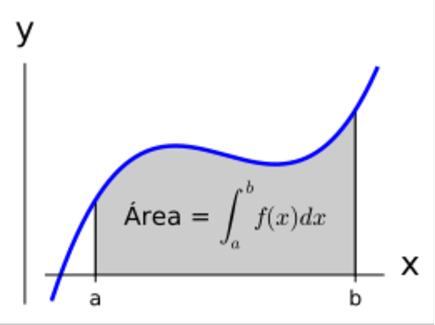
\includegraphics[width=\linewidth]{images/area-integral-definida}
\tcblower
\end{figureptx}%
\end{sbspanel}%
\end{sidebyside}%
%
\end{definition}
\begin{example}{}{x:example:ex1-area}%
Calcule a área da região limitada pelo gráfico de pelo gráfico de  \(f(x)=3x \), pelo eixo \(x\) e pela reta \(x=2\).%
\par\smallskip%
\noindent\textbf{\blocktitlefont Solução}.\hypertarget{g:solution:idp3}{}\quad{}\begin{sidebyside}{2}{0.0125}{0.0125}{0.025}%
\begin{sbspanel}{0.65}%
De acordo com a \hyperref[x:definition:def-area]{Definição~{\xreffont\ref{x:definition:def-area}}}, a integral definida de \(3x\) de \(0\) até \(2\) representa a área da região limitada pelo gráfico de \(f(x)=3x \), pelo eixo \(x\) e pela reta \(x=2\), como mostra a figura \hyperref[x:figure:figure-sage-exe1-area]{Figura~{\xreffont\ref{x:figure:figure-sage-exe1-area}}}. A região é triângular, com uma base de \(2\) unidades e altura de \(6\) unidades. Portanto, usando a fórmula da área do triângulo, temos%
\begin{align*}
\integrald{3x}{0}{2}{x} = \amp \frac{1}{2}(2)(6)=6 \text{.}
\end{align*}
%
\end{sbspanel}%
\begin{sbspanel}{0.3}%
\begin{figureptx}{Área entre o gráfico de \(f(x)=3x\), o eixo \(x\) e a reta \(x=2\)}{x:figure:figure-sage-exe1-area}{}%
\IfFileExists{images/sageplot-reta3x.pdf}%
{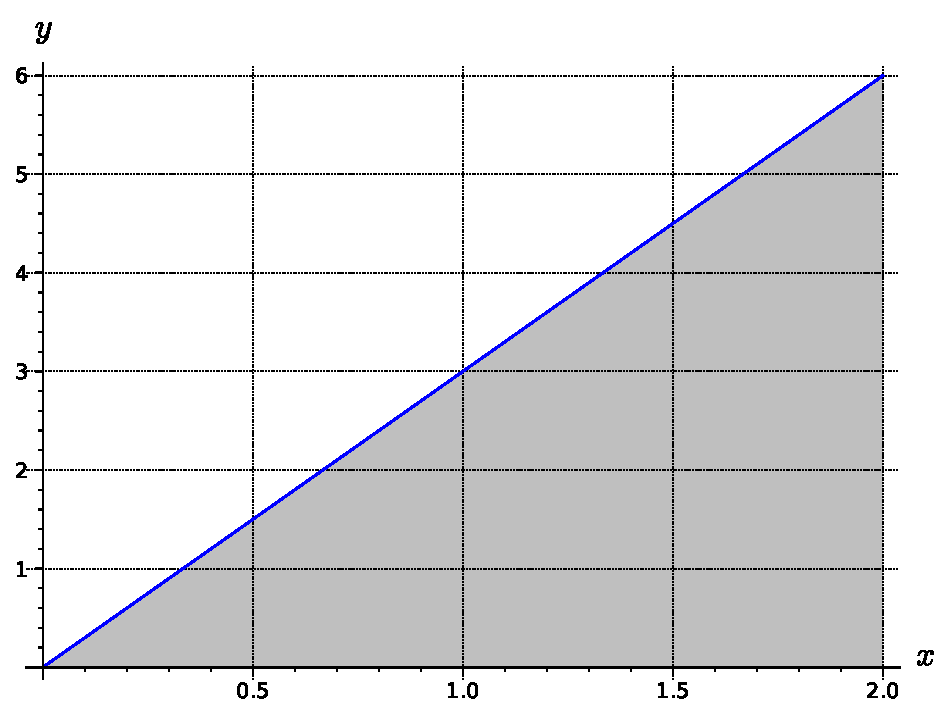
\includegraphics[width=\linewidth]{images/sageplot-reta3x.pdf}}%
{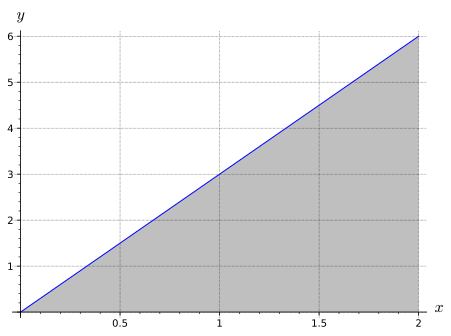
\includegraphics[width=\linewidth]{images/sageplot-reta3x.png}}
\tcblower
\end{figureptx}%
\end{sbspanel}%
\end{sidebyside}%
%
\end{example}
\begin{inlineexercise}{}{x:exercise:ex2-area}%
Calcule a integral definida de \(4x\) de \(0\) até \(3\), usando uma fórmula geométrica. Ilustre sua resposta com um gráfico apropriado.%
\par\smallskip%
\noindent\textbf{\blocktitlefont Dica}.\hypertarget{g:hint:idp4}{}\quad{}Revise \hyperref[x:example:ex1-area]{Exemplo~{\xreffont\ref{x:example:ex1-area}}}.%
\par\smallskip%
\noindent\textbf{\blocktitlefont Resposta}.\hypertarget{g:answer:idp5}{}\quad{}\(18\)%
\end{inlineexercise}%
\begin{technology}{Faça você mesmo.}{g:technology:idp6}%
Para visualizar a região sob o gráfico de um função \emph{não negativa} entre \(a\) e \(b\) se dirija até a calculadora gráfica abaixo e siga os seguintes passos:%
\begin{enumerate}
\item{}Em \(f(x)\), insira uma função contínua pelo menos no intervalo \([-10,10]\) ou em qualquer subintervalo deste. Por exemplo, \([0,1].\) Por padrão usamos a função \(f(x)=x^2\).%
\item{}Olhando para o gráfico, faça ajustes no intervalo para garantir que o gráfico de \(y=f(x)\), inserido no passo anterior, esteja sempre acima do eixo \(x\). (A função deve ser não negativa, lembra?)%
\item{}Marque a opção para mostrar a região pretendida.%
\end{enumerate}
Seguindo os passos acima você encontra a região cuja \terminology{área}  é dada por%
\begin{equation*}
\integrald{f(x)}{a}{b}{x}\text{.}
\end{equation*}
%
\begin{figureptx}{Região sob o gráfico de uma função}{x:figure:figure-interactive-numerical-integral}{}%
\centering
\setlength{\qrsize}{9em}
\setlength{\previewwidth}{\linewidth}
\addtolength{\previewwidth}{-\qrsize}
\begin{tcbraster}[raster columns=2, raster column skip=1pt, raster halign=center, raster force size=false, raster left skip=0pt, raster right skip=0pt]%
\begin{tcolorbox}[previewstyle, width=\previewwidth]%
\IfFileExists{images/interactive-numerical-integral-preview.png}%
{\includegraphics[width=0.80\linewidth,height=\qrsize,keepaspectratio]{images/interactive-numerical-integral-preview.png}}%
{\small{}Specify static image with \mono{@preview} attribute,\\Or create and provide automatic screenshot as \mono{images/interactive-numerical-integral-preview.png} via the \mono{mbx} script}%
\end{tcolorbox}%
\begin{tcolorbox}[qrstyle]%
{\hypersetup{urlcolor=black}\qrcode[height=\qrsize]{interactive-numerical-integral.html}}%
\end{tcolorbox}%
\end{tcbraster}%
\tcblower
\end{figureptx}%
\end{technology}
\begin{note}{}{g:note:idp7}%
Outra forma de introduzir a integral definida é através do processo de somas. Nesse caso, a região é dividida em um certo número de retângulos cuja a altura seja \(f(x)\). A  soma da área de cada retângulo definido dessa forma é denominada de \terminology{Soma de Riemann}. O limite da Soma de \emph{Riemann}, quando a base de cada retângulo se aproxima de zero, é também chamado de \terminology{integral definida}. Nas próximas seções daremos mais detalhes sobre essa abordagem.\end{note}
\end{subsectionptx}
%
%
\typeout{************************************************}
\typeout{Subseção 1.2 Teorema Fundamental do Cálculo}
\typeout{************************************************}
%
\begin{subsectionptx}{Teorema Fundamental do Cálculo}{}{Teorema Fundamental do Cálculo}{}{}{x:subsection:sec-TFC2}
\begin{theorem}{Teorema Fundamental do Cálculo - parte 1 (TFC1).}{}{x:theorem:thm-TFC1}%
Se \(f\) é contínua definida no intervalo \([a,b]\). Seja \(F(x)\) uma função definida, para todo \(x\) em \([a,b]\), por%
\begin{equation*}
F(x)=\integrald{f(t)}{a}{x}{t}\text{.}
\end{equation*}
Então \(F\) é contínua em \([a,b]\) e derivável em \((a,b)\). Além disso,%
\begin{equation*}
F'(x)=f(x),
\end{equation*}
para todo \(x\) em \((a,b)\).%
\begin{proof}{}{g:proof:idp8}
depois%
\end{proof}
\end{theorem}
\begin{example}{}{x:example:ex1-TFC1}%
Adicionar exemplo%
\par\smallskip%
\noindent\textbf{\blocktitlefont Solução}.\hypertarget{g:solution:idp9}{}\quad{}Adicionar solução%
\end{example}
\begin{example}{}{x:example:ex2-TFC1}%
Adicionar exemplo%
\par\smallskip%
\noindent\textbf{\blocktitlefont Solução}.\hypertarget{g:solution:idp10}{}\quad{}Adicionar solução%
\end{example}
\begin{inlineexercise}{}{x:exercise:exer1-TFC1}%
Adicionar autoavaliação%
\par\smallskip%
\noindent\textbf{\blocktitlefont Dica}.\hypertarget{g:hint:idp11}{}\quad{}Adicionar dica%
\par\smallskip%
\noindent\textbf{\blocktitlefont Resposta}.\hypertarget{g:answer:idp12}{}\quad{}Adicionar resposta%
\end{inlineexercise}%
\begin{inlineexercise}{}{x:exercise:exer2-TFC1}%
adicionar autovaliação%
\par\smallskip%
\noindent\textbf{\blocktitlefont Dica}.\hypertarget{g:hint:idp13}{}\quad{}Adicionar dica%
\par\smallskip%
\noindent\textbf{\blocktitlefont Resposta}.\hypertarget{g:answer:idp14}{}\quad{}Adicionar resposta%
\end{inlineexercise}%
\begin{theorem}{Teorema Fundamental do Cálculo - parte 2 (TFC2).}{}{x:theorem:thm-TFC}%
Se \(f\) é contínua no intervalo \([a,b]\), e  \(F\) é igual a \(f(x)\) para todo \(x\) em \([a,b]\), então%
\begin{gather*}
\integrald{f(x)}{a}{b}{x}= F(b) - F(a) \text{.}
\end{gather*}
%
\begin{proof}{}{g:proof:idp15}
mais adiante ...%
\end{proof}
\end{theorem}
Na \hyperref[x:definition:def-area]{Definição~{\xreffont\ref{x:definition:def-area}}} assumia-se que \(f\) era não negativa no intervalo fechado \([a, b]\). Assim, a integral definida era definida como uma área. Agora, a partir do \hyperref[x:theorem:thm-TFC]{Teorema Fundamental do Cálculo}, a definição pode ser estendida para incluir funções negativas em todo o intervalo fechado \([a, b]\) ou em parte dele. Especificamente, se \(f\) for qualquer função contínua em um intervalo \([a, b]\),  então a \terminology{integral definida} de \(f(x)\)  de \(a\) até \(b\)  é definida como%
\begin{equation*}
\integrald{f(x)}{a}{b}{x}= F(b) - F(a)\text{,}
\end{equation*}
em que \(F'(x)=f(x)\). Dessa forma, as \terminology{integral definidas} não representam necessariamente áreas e, portanto, podem ser negativas, positivas ou zero.%
\begin{assemblage}{Atenção.}{x:assemblage:assemblage-definida-indefinida}%
Há uma significativa diferença entre integral indefinida e integral definida. A \emph{integral indefinida}%
\begin{equation*}
\integral{f(x)}{x}
\end{equation*}
denota uma família de funções na qual cada membro é uma primitiva de \(f(x)\), enquanto a \emph{integral indefinida}%
\begin{equation*}
\integrald{f(x)}{a}{b}{x}
\end{equation*}
é um número.%
\end{assemblage}
\begin{example}{}{x:example:ex2-tfc}%
Usando o \hyperref[x:theorem:thm-TFC]{TFC}   resolva  a integral definida%
\begin{gather*}
\integrald{2x}{0}{2}{x} \text{.}
\end{gather*}
%
\par\smallskip%
\noindent\textbf{\blocktitlefont Solução}.\hypertarget{g:solution:idp16}{}\quad{}Note que \(F(x)=x^2\) é uma primitiva de \(2x\). Então, pelo \hyperref[x:theorem:thm-TFC]{TFC}, temos%
\begin{align*}
\integrald{2x}{0}{2}{x} \amp = 2^2 -  0^2 = 4 \text{.}
\end{align*}
%
\end{example}
\begin{inlineexercise}{}{x:exercise:exe2-TFC}%
Usando o \hyperref[x:theorem:thm-TFC]{TFC}   resolva  a integral%
\begin{gather*}
\integrald{4x}{0}{3}{x}.
\end{gather*}
%
\par\smallskip%
\noindent\textbf{\blocktitlefont Dica}.\hypertarget{g:hint:idp17}{}\quad{}Revise \hyperref[x:example:ex2-tfc]{Exemplo~{\xreffont\ref{x:example:ex2-tfc}}}.%
\par\smallskip%
\noindent\textbf{\blocktitlefont Resposta}.\hypertarget{g:answer:idp18}{}\quad{}18%
\end{inlineexercise}%
\begin{assemblage}{Notação útil.}{x:assemblage:assemblage-notacao}%
Quando usamos o Teorema Fundamental do Cálculo é util usar a notação%
\begin{gather*}
\integrald{f(x)}{a}{b}{x}=F(x)\biggr\rvert_a^b= F(b) - F(a).
\end{gather*}
%
\end{assemblage}
\begin{investigation}{Onde está a constante \(C\)?}{g:investigation:idp19}%
Revise o \hyperref[x:theorem:thm-TFC]{TFC} e justifique o "sumiço" da constante \(C\) que forma a primitiva \(F\).%
\end{investigation}%
\begin{assemblage}{Propriedades da integral definida.}{x:assemblage:assemblage-definida-propriedade}%
Sejam \(f\) e \(g\) contínuas no intervalo \([a,b]\) e \(k\) uma constante.%
\begin{enumerate}[label=\Roman*)]
\item\hypertarget{x:li:p-constante}{}\(\displaystyle \integrald{kf(x)}{a}{b}{x} = k \integrald{f(x)}{a}{b}{x}\)%
\item\hypertarget{x:li:p-soma}{}\(\displaystyle \integrald{\left[f(x)+ g(x)\right]}{a}{b}{x} = \integrald{f(x)}{a}{b}{x} + \integrald{g(x)}{a}{b}{x}\)%
\item\hypertarget{x:li:p-sub}{}\(\displaystyle \integrald{\left[f(x)- g(x)\right]}{a}{b}{x} = \integrald{f(x)}{a}{b}{x} - \integrald{g(x)}{a}{b}{x}\)%
\item\hypertarget{x:li:p-acb}{}\(\displaystyle \integrald{f(x)}{a}{b}{x} = \integrald{f(x)}{a}{c}{x} + \integrald{f(x)}{c}{b}{x} \quad a < c < b \)%
\item\hypertarget{x:li:p-aa-0}{}\(\displaystyle \integrald{f(x)}{a}{a}{x}=0 \)%
\item{}\(\displaystyle \integrald{f(x)}{b}{a}{x}=-\integrald{f(x)}{a}{b}{x}\)%
\end{enumerate}
%
\end{assemblage}
\begin{example}{Cálculo da área.}{x:example:ex3-area}%
Determine a área sob o gráfico de \(f(x)=x^2-1\) entre \(1\) e \(2\).%
\par\smallskip%
\noindent\textbf{\blocktitlefont Solução}.\hypertarget{g:solution:idp20}{}\quad{}A \hyperref[x:figure:fig-area1]{Figura~{\xreffont\ref{x:figure:fig-area1}}}  ilustra a área área desejada, cujo valor é obtido como a seguir:%
\begin{align*}
\text{Área}  \amp = \integrald{(x^2-1)}{1}{2}{x} \amp \amp \ct{Integral definida}\\
\amp =\left(\frac{x^3}{3}-x\right)\Biggr\rvert_1^2 \amp \amp \ct{Calcule a primitiva} \\
\amp = \left(\frac{2^3}{3}-2\right)- \left(\frac{1^3}{3}-1\right)  \amp \amp \ct{Aplique o} \, \hyperref[x:theorem:thm-TFC]{\text{TFC}} \\
\amp = \frac{4}{3} 
\end{align*}
Dessa forma, podemos dizer que a área da região é de \(\frac{4}{3}\). \begin{figureptx}{Região limitada por \(f(x)=x^2-1\), o eixo \(x\) e a reta \(x=2\).}{x:figure:fig-area1}{}%
\begin{image}{0.325}{0.35}{0.325}%
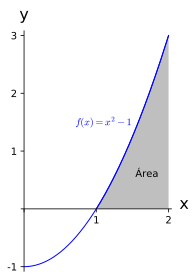
\includegraphics[width=\linewidth]{images/exemplo-area-1}
\end{image}%
\tcblower
\end{figureptx}%
%
\end{example}
\begin{inlineexercise}{}{x:exercise:exe3-area}%
Determine a área da região limitada pelo eixo \(x\), pelas retas \(x=2\), \(x=5\) e pelo gráfico de \(f(x)=x^2+1.\)%
\par\smallskip%
\noindent\textbf{\blocktitlefont Dica}.\hypertarget{g:hint:idp21}{}\quad{}Revise \hyperref[x:example:ex3-area]{Exemplo~{\xreffont\ref{x:example:ex3-area}}}.%
\par\smallskip%
\noindent\textbf{\blocktitlefont Resposta}.\hypertarget{g:answer:idp22}{}\quad{}42%
\end{inlineexercise}%
\begin{example}{Mais exemplos.}{x:example:ex5-integral-definida}%
Calcule as seguintes integrais definidas. \(\integrald{e^{2x}}{0}{2}{x}\)%
\par\smallskip%
\noindentUma primitiva de \(e^{2x}\) pode ser  \(F(x)=\frac{e^{2x}}{2}\). Então,%
\begin{align*}
\integrald{e^{2x}}{0}{2}{x}\amp = \frac{e^2x}{2} \Biggr\rvert_0^2 = 
\frac{1}{2}\left(e^4-e^0\right) \approx 26.79
\end{align*}
%
 \(\integrald{\frac{1}{x}}{3}{6}{x}\)%
\par\smallskip%
\noindentUma primitiva de \(\frac{1}{x}\) pode ser \(F(x)=\ln{|x|}\), e, já que \(3\leq x\leq 6\), podemos escrever \(F(x)=\ln{x}\). Assim,%
\begin{align*}
\integrald{\frac{1}{x}}{3}{6}{x} \amp = \ln{x}\Biggr\rvert_3^6 =\ln{6} - \ln{3} \\
\amp = \ln{\frac{6}{3}} = \ln{2} \approx 0.6931 
\end{align*}
%
 \(\integrald{-3\sqrt{t}}{1}{4}{t}\)%
\par\smallskip%
\noindentReescrevendo \(\sqrt{t}\) como \(t^{1/2}\) e aplicando a regra da potência encontramos \(F(x)=\frac{t^{3/2}}{3/2}\) como primitiva. Então,%
\begin{align*}
\integrald{-3\sqrt{t}}{1}{4}{t}\amp = -3\left(\frac{t^{3/2}}{3/2} \right)\Biggr\rvert_1^4 \amp \ct{Aplique o} \, \hyperref[x:theorem:thm-TFC]{\text{TFC}}.\\
\amp = -2x^{3/2}\Biggr\rvert_1^4 \amp \ct{Simplifique.}\\
\amp = -2(4^{3/2}-1^{3/2}) = -2(8-1)=-14
\end{align*}
%
%
\end{example}
\begin{inlineexercise}{}{x:exercise:exe5-log-exp}%
Calcule cada integral definida. \(\integrald{e^{-x}}{0}{1}{x}\)%
\par\smallskip%
\noindent\(F(x)= -e^{-x} \).%
\par\smallskip%
\noindentAproximadamente 0.6321.%
 \(\integrald{-\frac{4}{x}}{3}{6}{x}\)%
\par\smallskip%
\noindentRevise \hyperref[x:task:task-def-ln]{Tarefa~.{\xreffont\ref{x:task:task-def-ln}}}.%
\par\smallskip%
\noindent\(4\ln{(1/2)}\) ou aproximadamente  -2.772.%
%
\end{inlineexercise}%
\begin{example}{Função modular.}{x:example:ex6-integral-definida}%
Sobre função \(f(x)=|2x-1|\), resolva.%
Esboce a região sob o gráfico de \(f(x)\) de \(x=0\) até \(x=2\).%
\par\smallskip%
\noindent\begin{figureptx}{Região determinada por \(f(x)=|x-2|\), o eixo \(x\) e as reta \(x=0\) e \(x=2\)}{x:figure:figure-sage-exe6-area}{}%
\begin{image}{0.275}{0.45}{0.275}%
\IfFileExists{images/sageplot-ex6-madular.pdf}%
{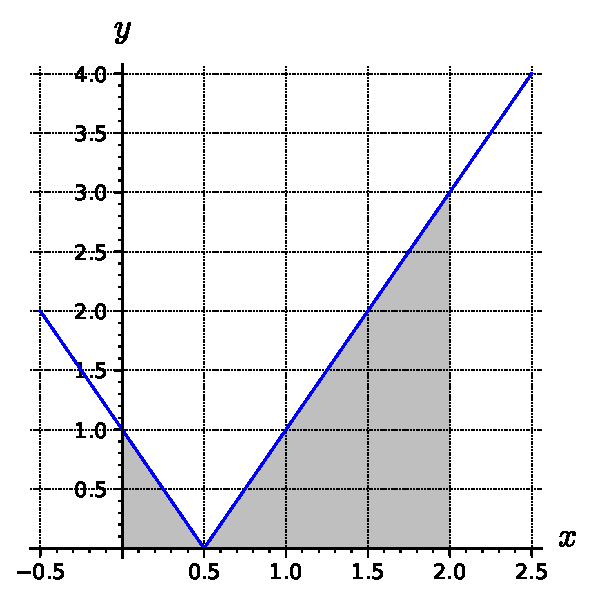
\includegraphics[width=\linewidth]{images/sageplot-ex6-madular.pdf}}%
{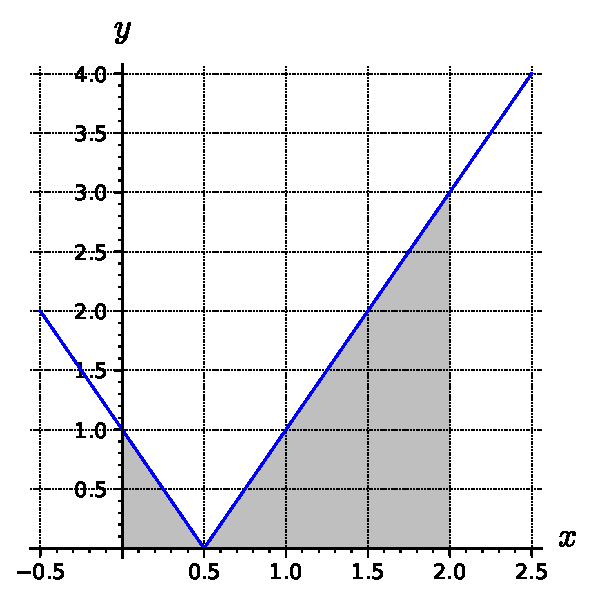
\includegraphics[width=\linewidth]{images/sageplot-ex6-madular.png}}
\end{image}%
\tcblower
\end{figureptx}%
%
Calcule \(\integrald{f(x)}{0}{2}{x}\).%
\par\smallskip%
\noindentA partir da definição de valor absoluto, o integrando \(|2x-1|\) pode ser escrito em duas partes, a saber:%
\begin{equation*}
|2x-1| = \begin{cases} -(2x-1), \amp x\lt 1/2 \\
2x-1, \amp x \geq 1/2 \end{cases}.
\end{equation*}
Usando \hyperlink{x:li:p-acb}{Item~{\xreffont IV}} das propriedades de integral definida, podemos reescrever a integral como duas outras de modo que a soma seja igual a integral desejada.%
\begin{align*}
\integrald{|2x-1|}{0}{2}{x}\amp = \integrald{-(2x-1)}{0}{1/2}{x} +  \integrald{(2x-1)}{1/2}{2}{x} \\
\amp = \left(-x^2+ x\right)\Biggr\rvert_0^{1/2} + \left(x^2-x\right)\Biggr\rvert_{1/2}^{2} \\
\amp = \left(-\frac{1}{4}+ \frac{1}{2}\right) - (0 +0) + (4-2)-\left(\frac{1}{4}-\frac{1}{2}\right)=\frac{5}{2} \text{.}
\end{align*}
%
\end{example}
\begin{activity}{Valor absoluto.}{g:activity:idp23}%
\begin{enumerate}[font=\bfseries,label=(\alph*),ref=\alph*]
\item\label{x:task:exe-a}Determine a região determinada pelo gráfico de \(f(x)=|x-2|\), pelas as retas \(x=0\) e \(x=5\) e o eixo \(x\).%
\par\smallskip%
\noindent\textbf{\blocktitlefont Resposta}.\hypertarget{g:answer:idp24}{}\quad{}\begin{image}{0.275}{0.45}{0.275}%
\IfFileExists{images/sageplot-ativ-madular.pdf}%
{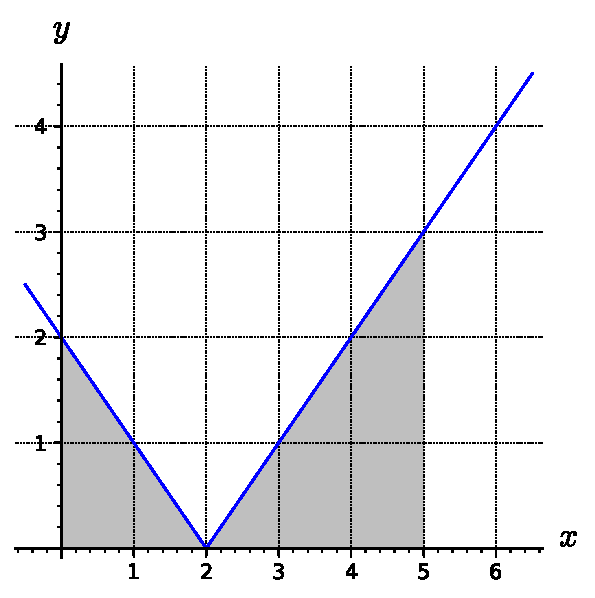
\includegraphics[width=\linewidth]{images/sageplot-ativ-madular.pdf}}%
{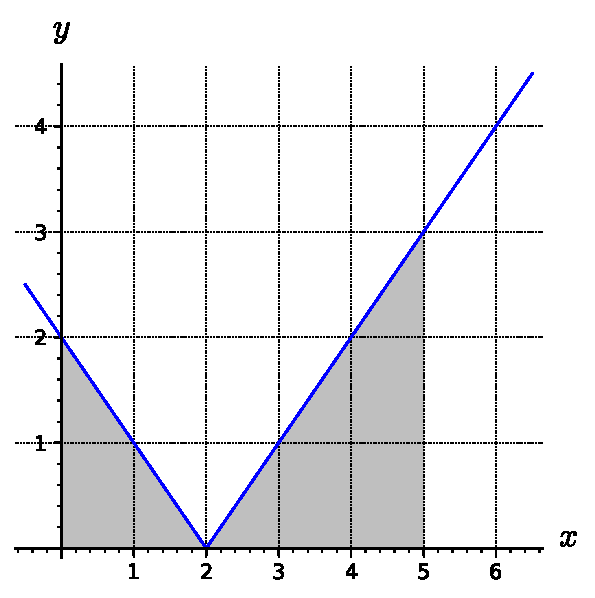
\includegraphics[width=\linewidth]{images/sageplot-ativ-madular.png}}
\end{image}%
%
\item\label{x:task:exe-b}Calcule a área da região descrita no item anterior usando fórmulas geométricas.%
\par\smallskip%
\noindent\textbf{\blocktitlefont Resposta}.\hypertarget{g:answer:idp25}{}\quad{}\(\frac{13}{2}\)%
\item\label{x:task:exe-c}Calcule  \(\integrald{|x-2|}{0}{5}{x}\) e compare com o item anterior.%
\par\smallskip%
\noindent\textbf{\blocktitlefont Resposta}.\hypertarget{g:answer:idp26}{}\quad{}\(\frac{13}{2}\)%
\end{enumerate}
\end{activity}%
\begin{investigation}{}{x:investigation:inv-propriedades}%
Use os recursos matemáticos apresentados até aqui para mostrar que as \hyperref[x:assemblage:assemblage-definida-propriedade]{Propriedades da integral definida} são verdadeiras.%
\end{investigation}%
\end{subsectionptx}
%
%
\typeout{************************************************}
\typeout{Subseção 1.3 Sugestão de Vídeos}
\typeout{************************************************}
%
\begin{subsectionptx}{Sugestão de Vídeos}{}{Sugestão de Vídeos}{}{}{x:subsection:subsec-videos-propriedades-e-TFC}
%
\begin{itemize}[label=\textbullet]
\item{}Propriedade da integral definida: \href{https://youtu.be/CF2XgyYsBFk}{trocando o sinal da integral}%
\item{}Propriedade da integral definida: \href{https://youtu.be/5JZUnWN5AQI}{somando áreas}%
\item{}Calculando área: \href{https://youtu.be/hwFbPNhzegE}{usando o gráfico I}%
\item{}Calculando área: \href{https://youtu.be/dM8HGLSq0RU}{usando o gráfico II}%
\item{}\href{https://youtu.be/Gv2W0WXMmhw}{Teorema Fundamental do Cálculo}%
\item{}Encontrando \href{https://youtu.be/wYiwhLne-oc}{\(\dfrac{\dd}{\dd x}\integrald{\sqrt{|\cos(t)|}}{x}{3}{t}\)}%
\item{}Encontrando \href{https://youtu.be/Gv2W0WXMmhw}{\(\dfrac{\dd}{\dd x}\integrald{\frac{\cos(t)}{t}}{x}{x^2}{t}\)}%
\item{}Calculando \href{}{integrais do tipo \(\integrald{kx^n}{a}{b}{x}\)}%
\item{}Calculando \href{https://youtu.be/k8ZYPiJzAN4}{\(\integrald{\frac{16-x^3}{x^3}}{-1}{-2}{x}\)}%
\item{}Calculando \href{https://youtu.be/VqBHvcTgCtc}{\(\integrald{\frac{6+x^2}{x^3}}{2}{4}{x}\) (envolve logaritmo)}%
\item{}Calculando \href{https://youtu.be/QzxlZhSpAFw}{\(\integrald{9\sin{x}}{\frac{11\pi}{2}}{6\pi}{x}\)}%
\item{}Calculando a integral  \href{https://youtu.be/tMZL9IuQN14}{\(\integrald{f(x)}{-1}{1}{x}  \) para \(f(x) = \begin{cases}
x+ 1, \amp  x \lt  0 \\
\cos(\pi x), \amp  x \geq 0.
\end{cases}\)}%
\item{}Calculando \href{https://youtu.be/WKef_JrXs-c}{\(\integrald{|x+2|}{-4}{0}{x}\)}%
\end{itemize}
\end{subsectionptx}
%
%
\typeout{************************************************}
\typeout{Subseção 1.4 Integrando funções com gráficos simétricos}
\typeout{************************************************}
%
\begin{subsectionptx}{Integrando funções com gráficos simétricos}{}{Integrando funções com gráficos simétricos}{}{}{x:subsection:subsec-simetria}
\begin{introduction}{}%
Gráficos de funções são úteis para analisar várias propriedades importantes. Diversas funções possuem  simetria em relação em relação ao eixo \(y\), como na \hyperref[x:figure:fig-par]{Figura~{\xreffont\ref{x:figure:fig-par}}} e outras apresentam simetria em relação a origem, como na \hyperref[x:figure:fig-impar]{Figura~{\xreffont\ref{x:figure:fig-impar}}}. No primeiro caso, a função é dita \terminology{par} e satisfaz \(f(-x)=f(x)\) em \([-a,a]\), e no segundo a função é dita \terminology{ímpar} e satisfaz \(f(-x)=-f(x)\) em \([-a,a]\).%
\end{introduction}%
\begin{figureptx}{Gráficos simétricos.}{g:figure:idp27}{}%
\begin{sidebyside}{2}{0.01}{0.01}{0.02}%
\begin{sbspanel}{0.48}[center]%
\begin{subfigureptx}{Simetria em relação ao eixo y}{x:figure:fig-par}{}%
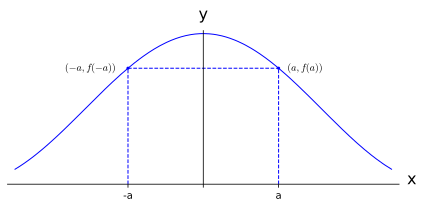
\includegraphics[width=\linewidth]{images/f-par}
\tcblower
\end{subfigureptx}%
\end{sbspanel}%
\begin{sbspanel}{0.48}[center]%
\begin{subfigureptx}{Simetria em relação a origem}{x:figure:fig-impar}{}%
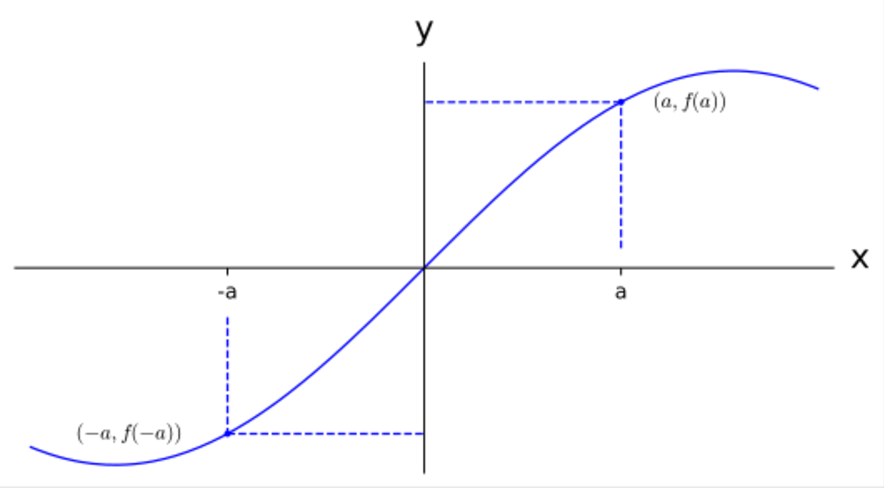
\includegraphics[width=\linewidth]{images/f-impar}
\tcblower
\end{subfigureptx}%
\end{sbspanel}%
\end{sidebyside}%
\tcblower
\end{figureptx}%
\begin{assemblage}{Integração com funções pares e ímpares.}{x:assemblage:assemblage-par-impar}%
%
\begin{enumerate}[label=\Roman*)]
\item\hypertarget{x:li:fact-par-1}{}Se \(f\) for uma função \terminology{par}, então \(\integrald{f(x)}{-a}{a}{x}=2\integrald{f(x)}{0}{a}{x}\)%
\item\hypertarget{x:li:fact-impar-2}{}Se \(f\) for uma função \terminology{ímpar}, então \(\integrald{f(x)}{-a}{a}{x}=0\)%
\end{enumerate}
%
\end{assemblage}
\begin{example}{}{x:example:ex-par-impar}%
Calcule a integral definida \(\integrald{x^2}{-2}{2}{x}\)%
\par\smallskip%
\noindentA função \(f(x)=x^2\) é par, pois \(x^2=(-x)^2\) para todo \(x\) em \([-2,2]\). Então, de acordo com o \hyperlink{x:li:fact-par-1}{Item~{\xreffont I}}, temos%
\begin{align*}
\integrald{x^2}{-2}{2}{x} \amp = 2\integrald{x^2}{0}{2}{x} \\
\amp = 2\cdot\frac{x^3}{3}\Biggr\rvert_0^{2} =2\cdot\frac{2^3}{3} - 2\cdot\frac{0^3}{3}=\frac{16}{3}\text{.}
\end{align*}
%
 \(\integrald{t^3}{-2}{2}{t}\)%
\par\smallskip%
\noindentA função \(t^3\) é ímpar, já que \(-t^3= (-t)^3\) para todo \(x\) em \([-2,2]\). Logo, de acordo com o \hyperlink{x:li:fact-impar-2}{Item~{\xreffont II}},%
\begin{equation*}
\integrald{t^3}{-2}{2}{t}=0\text{.}
\end{equation*}
%
%
\end{example}
\begin{inlineexercise}{}{x:exercise:exe7-par-impar}%
\(\integrald{t^4}{-1}{1}{t}\)%
\par\smallskip%
\noindentVerifique se \(t^4\) é par ou ímpar em \([-1,1]\) e depois  use  as propriedades da \hyperref[x:assemblage:assemblage-par-impar]{Integração com funções pares e ímpares}.%
\par\smallskip%
\noindent\(\frac{2}{5}\)%
 \(\integrald{x^5}{-1}{1}{x}\)%
\par\smallskip%
\noindentVerifique se \(x^5\) é par ou ímpar em \([-1,1]\) e depois  use as propriedades da \hyperref[x:assemblage:assemblage-par-impar]{Integração com funções pares e ímpares}.%
\par\smallskip%
\noindent0%
%
\end{inlineexercise}%
\begin{investigation}{Sobre a integral de funções pares e ímpares.}{x:investigation:act-par-impar}%
Use os recursos matemáticos apresentados até aqui para mostrar que o \hyperlink{x:li:fact-par-1}{Item~{\xreffont I}} e o \hyperlink{x:li:fact-impar-2}{Item~{\xreffont II}} são verdadeiros.%
\end{investigation}%
\begin{investigation}{Sobre a integral de funções pares e ímpares.}{x:investigation:act-par-impar2}%
Encontre uma justificativa geométrica para as afirmações \hyperlink{x:li:fact-par-1}{Item~{\xreffont I}\textendash{}{\xreffont II}}.%
\end{investigation}%
\end{subsectionptx}
%
%
\typeout{************************************************}
\typeout{Subseção 1.5 Integrais definidas por substituição}
\typeout{************************************************}
%
\begin{subsectionptx}{Integrais definidas por substituição}{}{Integrais definidas por substituição}{}{}{x:subsection:subsec-definida-subs}
\begin{introduction}{}%
Existem duas formas de encontrar o valor da integral definida por substituição. A primeira, convida você a determinar uma primitiva e então aplicar o \hyperref[x:theorem:thm-TFC]{Teorema Fundamental do Cálculo}. Enquanto na segunda é necessário  mudar os limites de integração de acordo com a substituição escolhida e, só depois, aplicar o teorema. O exemplo a seguir apresentamos duas soluções, cada uma ilustra uma das  possibilidades.%
\end{introduction}%
\begin{example}{}{x:example:ex4-area}%
Calcule a integral definida \(\integrald{(4x+1)^2}{0}{1}{x}\).%
\par\smallskip%
\noindent\textbf{\blocktitlefont Solução 1}.\hypertarget{g:solution:idp28}{}\quad{}Escolha \(u=4x+1\). Então, \(\frac{\dd u}{\dd x}=4\)  e \(\dd u= 4\dd x\). Assim, podemos afirmar que \(\frac{(4x+1)^3}{3}\) é uma primitiva para \((4x+1)^2\). Logo,%
\begin{align*}
\integrald{(4x+1)^2}{0}{1}{x}\amp = \integrald{\frac{1}{4}(4x+1)^2(4)}{0}{1}{x}  \amp \ct{Multiplique e divida por 4}.\\
\amp =\left(\frac{1}{4}\frac{(4x+1)^3}{3}\right)\Biggr\rvert_0^{1} \amp \ct{Mantenha os limites de integração originais}\\
\amp = \frac{1}{4}\left(\frac{(4\cdot 1 + 1)^3}{3} - \frac{(4\cdot 0 + 1)^3}{3} \right) \amp \ct{Aplique o }\, \hyperref[x:theorem:thm-TFC]{\text{TFC}} \\
\amp =\frac{1}{4}\left(\frac{5^3}{3}-\frac{1^3}{3}\right)\\
\amp = \frac{31}{3} 
\end{align*}
%
\par\smallskip%
\noindent\textbf{\blocktitlefont Solução 2}.\hypertarget{g:solution:idp29}{}\quad{}Escolha \(u=4x+1\). Então, \(\frac{\dd u}{\dd x}=4\)  e \(\dd u= 4\dd x\). Para encontrar os novos limites de integração, observamos que quando \(x=0\), temos \(u=1\), por outro lado, para \(x=1\), obtemos \(u=5\). Logo,%
\begin{align*}
\integrald{(4x+1)^2}{0}{1}{x}\amp = \frac{1}{4}\integrald{u^2}{1}{5}{u} \amp \ct{Multiplique e divida por 4}\\
\amp = \frac{1}{4}\frac{u^3}{3}\Biggr\rvert_1^{5} \amp \ct{Mudança dos limites de integração}\\
\amp = \frac{1}{4}\left(\frac{5^3}{3}-\frac{1^3}{3}\right) \amp \ct{Aplique o }\, \hyperref[x:theorem:thm-TFC]{\text{TFC}}\\
\amp = \frac{31}{3}
\end{align*}
%
\end{example}
\begin{inlineexercise}{}{x:exercise:exe4-integral-definida}%
Calcule a integral definida \(\integrald{(2t+3)^3}{0}{1}{t}\).%
\par\smallskip%
\noindent\textbf{\blocktitlefont Dica}.\hypertarget{g:hint:idp30}{}\quad{}Escolha a substituição  \(u=2t+3\).%
\par\smallskip%
\noindent\textbf{\blocktitlefont Resposta}.\hypertarget{g:answer:idp31}{}\quad{}68%
\end{inlineexercise}%
\begin{assemblage}{Roteiro para encontrar integrais definidas por substituição.}{x:assemblage:assemblage-roteiro-subs-definida-integral}%
%
\begin{itemize}[label=\textbullet]
\item{}Use o método de substituição para encontrar uma primitiva em termos da variável original. Aplique o  \hyperref[x:theorem:thm-TFC]{Teorema Fundamental do Cálculo} utilizando os limites de integração originais; \terminology{ou}%
\item{}Escolha uma substituição adequada e converta os limites de integração originais em termos da nova variável. Aplique o \hyperref[x:theorem:thm-TFC]{Teorema Fundamental do Cálculo} sem converter a primitiva em termos da variável original.%
\end{itemize}
%
\end{assemblage}
\begin{note}{}{g:note:idp32}%
Embora as duas maneiras apresentadas para encontrar integrais definidas, por substituição, funcionem. É comum, por geralmente simplificar os cálculo, fazer uso da mudança dos limites de integração para a nova variável.\end{note}
\begin{inlineexercise}{}{x:exercise:exer-defi-subs1}%
Resolva a integral \(\integrald{\sqrt{2x+1}}{-\frac{1}{2}}{1}{x}\) usando as duas opções apresentadas no \hyperref[x:assemblage:assemblage-roteiro-subs-definida-integral]{Roteiro para encontrar integrais definidas por substituição}.%
\par\smallskip%
\noindent\textbf{\blocktitlefont Dica}.\hypertarget{g:hint:idp33}{}\quad{}Escolha a substituição \(u=2x+1\).%
\par\smallskip%
\noindent\textbf{\blocktitlefont Resposta}.\hypertarget{g:answer:idp34}{}\quad{}\(\sqrt{3}\)%
\end{inlineexercise}%
\begin{example}{}{x:example:exer-defi-subs2}%
Calcule  \(\integrald{xe^{x^2}}{0}{2}{x}\).%
\par\smallskip%
\noindent\textbf{\blocktitlefont Solução}.\hypertarget{g:solution:idp35}{}\quad{}Escolha \(u=x^2\). Então, \(\frac{\dd u}{\dd x}=2x\)  e \(\dd u= 2x\dd x\). Quando \(x=0\), \(u=0\), e, quando \(x=2\), \(u=4\). Logo,%
\begin{align*}
\integrald{xe^{x^2}}{0}{2}{x}\amp = \integral{\frac{1}{2}e^u}{u} = \frac{1}{2}e^u \Biggr\rvert_0^{4}\\
\amp = \frac{1}{2}\left(e^4-e^0\right)=\frac{1}{2}(e^4-1)\\
\amp \approx 26.79 \text{.}
\end{align*}
%
\end{example}
\begin{inlineexercise}{}{g:exercise:idp36}%
Calcule \(\integrald{2xe^{x^2}}{1}{2}{x}\).%
\par\smallskip%
\noindent\textbf{\blocktitlefont Dica}.\hypertarget{g:hint:idp37}{}\quad{}Revise \hyperref[x:example:exer-defi-subs2]{Exemplo~{\xreffont\ref{x:example:exer-defi-subs2}}}.%
\par\smallskip%
\noindent\textbf{\blocktitlefont Resposta}.\hypertarget{g:answer:idp38}{}\quad{}\(e^4 - e \approx 51.87\)%
\end{inlineexercise}%
\begin{example}{}{x:example:ex-defi-subs3}%
Calcule \(\integrald{\frac{\tan{t}}{\cos^2{t}}}{0}{\frac{\pi}{4}}{t}\).%
\par\smallskip%
\noindent\textbf{\blocktitlefont Solução}.\hypertarget{g:solution:idp39}{}\quad{}Escolha \(u=\tan{t}\). Então, \(\frac{\dd u}{\dd t}=(1/\cos^2{t})\)  e \(\dd u= (1/\cos^2{t})\dd t\). Quando \(t=0\), \(u=\tan{0}=0\), e, quando, \(x=\pi/4\), \(u=\tan{\pi/4}=1\). Portanto,%
\begin{align*}
\integrald{\frac{\tan{t}}{\cos^2{t}}}{0}{\frac{\pi}{4}}{t}\amp = \integrald{\tan{t}\cdot\left(\frac{1}{\cos^2{t}}\right)}{0}{\frac{\pi}{4}}{t}\\
\amp =  \integrald{u}{0}{1}{u} = \frac{u^2}{2} \Biggr\rvert_0^{1} = \left(\frac{1^2}{2}-\frac{0^2}{2}\right) \\
\amp = \frac{1}{2} \text{.}
\end{align*}
%
\end{example}
\begin{inlineexercise}{}{g:exercise:idp40}%
Refaça o \hyperref[x:example:ex-defi-subs3]{Exemplo~{\xreffont\ref{x:example:ex-defi-subs3}}} fazendo a substituição \(u=\cos{t}\). Conclua que embora o resultado final seja o mesmo, essa escolha torna o problema mais complicado.%
\end{inlineexercise}%
\begin{example}{}{x:example:ex-defi-subs4}%
Calcule \(\integrald{\frac{1}{5-x}}{1}{3}{x}\).%
\par\smallskip%
\noindent\textbf{\blocktitlefont Solução}.\hypertarget{g:solution:idp41}{}\quad{}A escolha u=5-x, fornece \(\dd u=(-1)\dd x \). Além disso, quando \(x=1\), \(u=4\), e , quendo \(x=3\), \(u=2\). Então,%
\begin{align*}
\integrald{\frac{1}{5-x}}{1}{3}{x} \amp  = \integrald{-\frac{1}{u}}{4}{2}{u}\\
\amp = -\ln{u}\Biggr\rvert_4^{2}  = - (\ln{2}-\ln{4})\\
\amp = \ln{\frac{4}{2}} = \ln{2} \approx 0,6931  \text{.}
\end{align*}
%
\end{example}
\begin{inlineexercise}{}{x:exercise:exer-subs-02}%
Calcule \(\integrald{\frac{1}{(3-5x)^2}}{1}{3}{x}\).%
\par\smallskip%
\noindent\textbf{\blocktitlefont Dica}.\hypertarget{g:hint:idp42}{}\quad{}Escolha a substituição \(u=3-5x\).%
\par\smallskip%
\noindent\textbf{\blocktitlefont Resposta}.\hypertarget{g:answer:idp43}{}\quad{}\(\frac{1}{12}\)%
\end{inlineexercise}%
\begin{example}{}{x:example:ex-defi-subs5}%
Calcule \(\integrald{\frac{\ln{x}}{x}}{1}{e}{x}\).%
\par\smallskip%
\noindent\textbf{\blocktitlefont Solução}.\hypertarget{g:solution:idp44}{}\quad{}Fazendo \(u=\ln{u}\), obtemos \(\frac{\dd u}{\dd x} = 1/x\). Então  \(\dd u = (1/x)\dd x\). Quando \(x=1\), \(u=\ln{1}=0\), e, quando \(x=e\) , \(u=\ln{e}=1\). Assim,%
\begin{align*}
\integrald{\frac{\ln{x}}{x}}{1}{e}{x}\amp = \integrald{u}{0}{1}{u} = \frac{u^2}{2}\Biggr\rvert_0^{1} \\
\amp = \left(\frac{1^2}{2} -\frac{0^2}{2}\right)=\frac{1}{2} \text{.}
\end{align*}
%
\end{example}
\begin{inlineexercise}{}{x:exercise:exer-subs-03}%
Calcule \(\integrald{\frac{1}{x\sqrt{\ln{x}}}}{e}{e^4}{x}\).%
\par\smallskip%
\noindent\textbf{\blocktitlefont Dica}.\hypertarget{g:hint:idp45}{}\quad{}Escolha a substituição \(u=\ln{x}\).%
\par\smallskip%
\noindent\textbf{\blocktitlefont Resposta}.\hypertarget{g:answer:idp46}{}\quad{}2%
\end{inlineexercise}%
\end{subsectionptx}
%
%
\typeout{************************************************}
\typeout{Subseção 1.6 Sugestão de Vídeos}
\typeout{************************************************}
%
\begin{subsectionptx}{Sugestão de Vídeos}{}{Sugestão de Vídeos}{}{}{x:subsection:subsec-videos-substituicao}
%
\begin{itemize}[label=\textbullet]
\item{}Resolvendo \href{https://youtu.be/nxj7iaQlKws}{\(\integrald{(2x(x^2+1)^3)}{1}{2}{x}\)}%
\item{}Resolvendo \href{https://youtu.be/VldmYmPi30M}{\(\integrald{x^{2}2^{x^3}}{0}{1}{x}\)}%
\end{itemize}
\end{subsectionptx}
%
%
\typeout{************************************************}
\typeout{Subseção 1.7 Calculando integrais definidas com SageMath}
\typeout{************************************************}
%
\begin{subsectionptx}{Calculando integrais definidas com SageMath}{}{Calculando integrais definidas com SageMath}{}{}{x:subsection:subsec-sage}
\begin{introduction}{}%
No Sage, usando o comando \mono{integral(f, (x, a, b))} é possível calcular a integral definida de \(f(x)\) de \(a\) até \(b\).%
\end{introduction}%
\begin{technology}{Faça você mesmo.}{g:technology:idp47}%
\leavevmode%
\begin{sageinput}
integral(x^2, (x, -1, 1))
\end{sageinput}
\begin{sageoutput}
2/3
\end{sageoutput}
Se a função estiver definida em uma variável simbólica diferente de \(x\), é necessário proceder de uma das formas a seguir:%
\begin{enumerate}
\item{}Substituir essa variável original por \(x\) quando for inserir o comando na célula.%
\item{}Definir a nova variável usando comando \mono{var()}.%
\end{enumerate}
%
\par
Logo abaixo vamos cálcular a integral \(\integrald{t^5}{-1}{1}{t}\) de ambas as formas.%
\begin{paragraphs}{Usando a variável \(x\).}{g:paragraphs:idp48}%
\leavevmode%
\begin{sageinput}
integral(x^5, (x, -1, 1))
\end{sageinput}
\begin{sageoutput}
0
\end{sageoutput}
\end{paragraphs}%
\begin{paragraphs}{Usando a variável apresentada no problema.}{g:paragraphs:idp49}%
\leavevmode%
\begin{sageinput}
t =  var('t')
integral(t^5, (t, -1, 1))
\end{sageinput}
\begin{sageoutput}
0
\end{sageoutput}
\end{paragraphs}%
\end{technology}
\begin{activity}{}{x:activity:sage-integral-definida}%
Utilize a célular abaixo para calcular as integrais dos exemplos desta seção.%
\begin{sageinput}

\end{sageinput}
\begin{sageoutput}
(for static output)
\end{sageoutput}
\end{activity}%
\end{subsectionptx}
%
%
\typeout{************************************************}
\typeout{Exercícios 1.8 Exercícios}
\typeout{************************************************}
%
\begin{exercises-subsection}{Exercícios}{}{Exercícios}{}{}{x:exercises:exercises-integral-definida}
\begin{divisionexercise}{1}{}{}{g:exercise:idp50}%
Encontre a área da região sob a curva \(y = 2 - 4 x^2\) e acima do eixo \(x\).%
\par
área = \fillin{6.818181818181818}%
\par\smallskip%
\noindent\textbf{\blocktitlefont Resposta}.\hypertarget{g:answer:idp51}{}\quad{}\(1.88561808316413\)%
\par\smallskip%
\noindent\textbf{\blocktitlefont Solução}.\hypertarget{g:solution:idp52}{}\quad{}Solução%
\par
A função que estamos considerando é%
\begin{sidebyside}{1}{0.416666666666667}{0.416666666666667}{0}%
\begin{sbspanel}{0.166666666666667}%
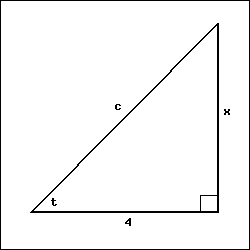
\includegraphics[width=\linewidth]{images/webwork-1-image-1.png}
\end{sbspanel}%
\end{sidebyside}%
\par
\emph{(Clique no gráfico para uma versão maior.)}%
\par
A área que queremos está acima do eixo \(x\) e sob o gráfico da função. As inteseções com o eixo \(x\) são o lugar onde \(y = 2 - 4 x^2 = 0\), que está em \(x = \pm\sqrt{\frac{2}{4}}\), então precisamos encontrar%
\begin{equation*}
\int_{-\sqrt{\frac{2}{4}}}^{\sqrt{\frac{2}{4}}} (2 - 4 x^2) dx \approx 1.885.
\end{equation*}
Podemos localizar a área de várias maneiras, a mais fácil delas é usar uma calculadora gráfica. Por exemplo, o Geogebra.%
\end{divisionexercise}%
\begin{divisionexercise}{2}{}{}{g:exercise:idp53}%
Encontre a área da região sob a curva \(y = 3 x^3 - 3\) e acima do eixo \(x\), para \(3 \le x \le 7\).%
\par
área = \fillin{6.818181818181818}%
\par\smallskip%
\noindent\textbf{\blocktitlefont Resposta}.\hypertarget{g:answer:idp54}{}\quad{}\(1728\)%
\par\smallskip%
\noindent\textbf{\blocktitlefont Solução}.\hypertarget{g:solution:idp55}{}\quad{}Solução%
\par
A função que estamos considerando é%
\begin{sidebyside}{1}{0.416666666666667}{0.416666666666667}{0}%
\begin{sbspanel}{0.166666666666667}%
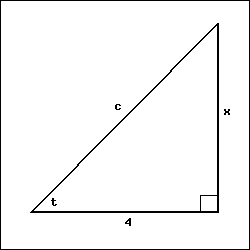
\includegraphics[width=\linewidth]{images/webwork-2-image-1.png}
\end{sbspanel}%
\end{sidebyside}%
\par
\emph{(Clique no gráfico para uma versão maior.)}%
\par
A área que queremos é aquela acima do eixo \(x\) e sob o gráfico da função, para \(3 \le x \le 7\). Portanto, precisamos encontrar%
\begin{equation*}
\int_{3}^{7} (3 x^3 - 3) dx \approx 1728.
\end{equation*}
Podemos localizar a área de várias maneiras, a mais fácil delas é usar uma calculadora gráfica, como o GeoGebra.%
\end{divisionexercise}%
\begin{divisionexercise}{3}{}{}{g:exercise:idp56}%
Esboce e encontre a área da região abaixo do intervalo \([-5, -4]\) e acima da curva \(y = \frac{x^{3}}{16}\).%
\par
área = \fillin{9.090909090909092}%
\par\smallskip%
\noindent\textbf{\blocktitlefont Resposta}.\hypertarget{g:answer:idp57}{}\quad{}\({\textstyle\frac{369}{64}}\)%
\par\smallskip%
\noindent\textbf{\blocktitlefont Solução}.\hypertarget{g:solution:idp58}{}\quad{}Solução%
\par
Traçando o gráfico, vemos que a região necessária tem:%
\par
Área \(= -\displaystyle \int^{-4}_{-5} \frac{x^{3}}{16} \;dx =  -\left[\frac{x^{4}}{64} \right]^{-4} _{-5} =-(4-{\textstyle\frac{625}{64}})={\textstyle\frac{369}{64}}\)%
\par
(Clique na imagem para ampliá-la)%
\begin{sidebyside}{1}{0.416666666666667}{0.416666666666667}{0}%
\begin{sbspanel}{0.166666666666667}%
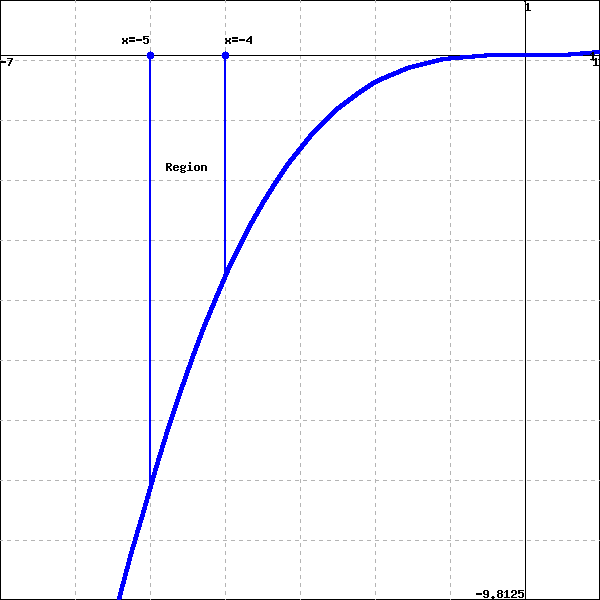
\includegraphics[width=\linewidth]{images/webwork-3-image-1.png}
\end{sbspanel}%
\end{sidebyside}%
\par
\(y=f(x)\)%
\end{divisionexercise}%
\begin{divisionexercise}{4}{}{}{g:exercise:idp59}%
Use o Teorema Fundamental do Cálculo para determinar o valor de \(b\) se a área sob o gráfico de \(f(x) = 6 x\) entre \(x = 1\) e \(x = b\) é igual a \(144\). Assuma \(b>1\).%
\par
\(b =\) \fillin{6.818181818181818}%
\par\smallskip%
\noindent\textbf{\blocktitlefont Resposta}.\hypertarget{g:answer:idp60}{}\quad{}\(7\)%
\par\smallskip%
\noindent\textbf{\blocktitlefont Solução}.\hypertarget{g:solution:idp61}{}\quad{}Solução%
\par
A área sob \(f(x) = 6 x\) entre \(x=1\) e \(x = b\) é dada por \(\int_1^b (6 x) dx\).  Usando o Teorema Fundamental para avaliar o integral:%
\begin{equation*}
\hbox{Area } = 3 x^2 \bigg|_1^b = 3 b^2 - 3.
\end{equation*}
Uma vez que a área é 144, temos%
\begin{equation*}
3 b^2 - 3 = 144,
\end{equation*}
logo%
\begin{equation*}
3 b^2 = 147,
\end{equation*}
e assim%
\begin{equation*}
b^2 = 49,\quad\hbox{ou}\quad b = \pm 7.
\end{equation*}
Já que \(b\) é maior que  1, obtemos \(b = 7\).%
\end{divisionexercise}%
\begin{divisionexercise}{5}{}{}{g:exercise:idp62}%
Determine as integrais definidas:%
\par
a) \(\displaystyle\int_{1}^{6} \dfrac{1}{x} \, dx =\) \fillin{6.818181818181818}%
\par
b) \(\displaystyle\int_{1}^{4} \dfrac{1}{x^2} \, dx =\) \fillin{6.818181818181818}%
\par
c) \(\displaystyle\int_{1}^{8} \dfrac{1}{x^{6}} \, dx =\) \fillin{6.818181818181818}%
\par
d) \(\displaystyle\int_{0}^{8} x^2 \, dx =\) \fillin{6.818181818181818}%
\par
e) \(\displaystyle\int_{0}^{1} x^{45} \, dx =\) \fillin{6.818181818181818}%
\par\smallskip%
\noindent\textbf{\blocktitlefont Resposta 1}.\hypertarget{g:answer:idp63}{}\quad{}\(1.79175946922805\)%
\par\smallskip%
\noindent\textbf{\blocktitlefont Resposta 2}.\hypertarget{g:answer:idp64}{}\quad{}\(0.75\)%
\par\smallskip%
\noindent\textbf{\blocktitlefont Resposta 3}.\hypertarget{g:answer:idp65}{}\quad{}\(0.199993896484375\)%
\par\smallskip%
\noindent\textbf{\blocktitlefont Resposta 4}.\hypertarget{g:answer:idp66}{}\quad{}\(170.666666666667\)%
\par\smallskip%
\noindent\textbf{\blocktitlefont Resposta 5}.\hypertarget{g:answer:idp67}{}\quad{}\(0.0217391304347826\)%
\par\smallskip%
\noindent\textbf{\blocktitlefont Solução}.\hypertarget{g:solution:idp68}{}\quad{}\alert{Solução:}%
\par
Use o Teorema Fundamental do Cálculo.%
\begin{equation*}
\begin{array}{rcl}
\displaystyle \int_{1}^{6} \dfrac{1}{x} \, dx \amp =\amp 
\left(\ln |x| \right) \Big|_{1}^{6}\\
\amp =\amp  \ln(6) - \ln(1)\\
\amp =\amp  \ln 6
\end{array}
\end{equation*}
%
\par
%
\begin{equation*}
\begin{array}{rcl}
\displaystyle \int_{1}^{4} \dfrac{1}{x^2} \, dx
\amp =\amp  \left( -\dfrac{1}{x} \right) \Big|_{1}^{4}\\
\amp =\amp  -\dfrac{1}{4} + 1
\amp =\amp  0.75
\end{array}
\end{equation*}
%
\par
%
\begin{equation*}
\begin{array}{rcl}
\displaystyle \int_{1}^{8} \dfrac{1}{x^{6}} \, dx \amp =\amp 
\left(-\dfrac{x^{-5}}{5} \right) \Big|_{1}^{8}\\
\amp \amp \\
\amp =\amp  -\dfrac{(8)^{-5}}{5} + \dfrac{1}{5} \\
\amp \amp \\
\amp =\amp  0.199994
\end{array}
\end{equation*}
%
\par
%
\begin{equation*}
\begin{array}{rcl}
\displaystyle \int_{0}^{8} x^2 \, dx
\amp =\amp  \left( \dfrac{x^3}{3} \right) \Big|_{0}^{8}\\
\amp \amp \\
\amp =\amp  \dfrac{(8)^3}{3} - 0\\
\amp \amp \\
\amp =\amp  170.667
\end{array}
\end{equation*}
%
\par
%
\begin{equation*}
\begin{array}{rcl}
\displaystyle \int_{0}^{1} x^{45} \, dx
\amp =\amp  \left( \dfrac{x^{46}}{46} \right) \Big|_{0}^{1}\\
\amp \amp \\
\amp =\amp  \dfrac{(1)^{46}}{46} - 0\\
\amp \amp \\
\amp =\amp  \dfrac{1}{46}
\end{array}
\end{equation*}
%
\end{divisionexercise}%
\begin{divisionexercise}{6}{}{}{g:exercise:idp69}%
Determine as integrais definidas:%
\par
a) \(\displaystyle\int_{\pi/2}^{\pi} -11 \cos x \, dx =\) \fillin{6.818181818181818}%
\par
b) \(\displaystyle\int_{0}^{\pi/4} 5 \sec^2 \theta \, d\theta =\) \fillin{6.818181818181818}%
\par
c) \(\displaystyle\int_{\pi/6}^{\pi/3} 13 \csc t \cot t \, dt =\) \fillin{6.818181818181818}%
\par\smallskip%
\noindent\textbf{\blocktitlefont Resposta 1}.\hypertarget{g:answer:idp70}{}\quad{}\(11\)%
\par\smallskip%
\noindent\textbf{\blocktitlefont Resposta 2}.\hypertarget{g:answer:idp71}{}\quad{}\(5\)%
\par\smallskip%
\noindent\textbf{\blocktitlefont Resposta 3}.\hypertarget{g:answer:idp72}{}\quad{}\(10.9888930010697\)%
\par\smallskip%
\noindent\textbf{\blocktitlefont Solução}.\hypertarget{g:solution:idp73}{}\quad{}\alert{Solução:}%
\par
Use o Teorema Fundamental do Cálculo.%
\begin{equation*}
\begin{array}{rcl}
\displaystyle \int_{\pi/2}^{\pi} -11 \cos x \, dx \amp =\amp 
\left(-11 \sin x \right) \Big|_{\pi/2}^{\pi}\\
\amp =\amp  \left(-11 \sin \pi\right) -  \left(-11 \sin (\pi/2)\right)\\
\amp =\amp  11
\end{array}
\end{equation*}
%
\par
%
\begin{equation*}
\begin{array}{rcl}
\displaystyle \int_{0}^{\pi/4} 5 \sec^2 \theta \, d\theta 
\amp =\amp  \left( 5\tan \theta \right) \Big|_{0}^{\pi/4}\\
\amp =\amp  \left( 5\tan(\pi/4)\right) -
\left( 5\tan 0\right)\\
\amp =\amp  5
\end{array}
\end{equation*}
%
\par
%
\begin{equation*}
\begin{array}{rcl}
\displaystyle \int_{\pi/6}^{\pi/3} 13 \csc t \cot t \, dt \amp =\amp 
\left(-13 \csc t \right) \Big|_{\pi/6}^{\pi/3}\\
\amp =\amp  \left(\dfrac{-13}{\sin (\pi/3)}\right) - 
\left(\dfrac{-13}{\sin(\pi/6)}
\right)\\
\amp =\amp  -\dfrac{26}{\sqrt{3}} + 26
\end{array}
\end{equation*}
%
\end{divisionexercise}%
\begin{divisionexercise}{7}{}{}{g:exercise:idp74}%
Determine as integrais definidas:%
\par
a) \(\displaystyle\int_{0}^{25} \sqrt{t} \, dt =\) \fillin{6.818181818181818}%
\par
b) \(\displaystyle\int_{4}^{9} \dfrac{1}{\sqrt{z}} \, dz =\) \fillin{6.818181818181818}%
\par
c) \(\displaystyle\int_{1}^{8} \sqrt[3]{x} \, dx =\) \fillin{6.818181818181818}%
\par\smallskip%
\noindent\textbf{\blocktitlefont Resposta 1}.\hypertarget{g:answer:idp75}{}\quad{}\(83.3333333333333\)%
\par\smallskip%
\noindent\textbf{\blocktitlefont Resposta 2}.\hypertarget{g:answer:idp76}{}\quad{}\(2\)%
\par\smallskip%
\noindent\textbf{\blocktitlefont Resposta 3}.\hypertarget{g:answer:idp77}{}\quad{}\(11.25\)%
\par\smallskip%
\noindent\textbf{\blocktitlefont Solução}.\hypertarget{g:solution:idp78}{}\quad{}\alert{Solução:}%
\par
Use o Teorema Fundamental do Cálculo.%
\begin{equation*}
\begin{array}{rcl}
\displaystyle \int_{0}^{25} \sqrt{t} \, dt \amp =\amp 
\left(\dfrac{2t^{3/2}}{3} \right) \Big|_{0}^{25}\\
\amp \amp \\
\amp =\amp  \dfrac{2(25)^{3/2}}{3} -  \dfrac{2(0)^{3/2}}{3} \\
\amp \amp \\
\amp =\amp  \dfrac{250}{3}\\
\amp =\amp  83.3333
\end{array}
\end{equation*}
%
\par
%
\begin{equation*}
\begin{array}{rcl}
\displaystyle \int_{4}^{9} \dfrac{1}{\sqrt{z}} \, dz
\amp =\amp  \left( 2\sqrt{z} \right) \Big|_{4}^{9}\\
\amp =\amp  2\sqrt{9} - 2\sqrt{4}\\
\amp =\amp  2
\end{array}
\end{equation*}
%
\par
%
\begin{equation*}
\begin{array}{rcl}
\displaystyle \int_{1}^{8} \sqrt[3]{x} \, dx \amp =\amp 
\left(\dfrac{3x^{4/3}}{4} \right) \Big|_{1}^{8}\\
\amp \amp \\
\amp =\amp  \dfrac{3(8)^{4/3}}{4} -  \dfrac{3(1)^{4/3}}{4} \\
\amp \amp \\
\amp =\amp  \dfrac{45}{4}\\
\amp =\amp  11.25
\end{array}
\end{equation*}
%
\end{divisionexercise}%
\begin{divisionexercise}{8}{}{}{g:exercise:idp79}%
Determine \(\displaystyle \int_{0}^{5} \!\left( 2 e^x+5\cos x\right)  \, dx =\) \fillin{9.090909090909092}%
\par\smallskip%
\noindent\textbf{\blocktitlefont Resposta}.\hypertarget{g:answer:idp80}{}\quad{}\(290.032\)%
\end{divisionexercise}%
\begin{divisionexercise}{9}{}{}{g:exercise:idp81}%
Calcule \(\displaystyle\int_{1}^{\,4} {\sqrt{t}(10 + t)}\,dt =\)%
\par\smallskip%
\noindent\textbf{\blocktitlefont Resposta}.\hypertarget{g:answer:idp82}{}\quad{}\(59.0666666666667\)%
\end{divisionexercise}%
\begin{divisionexercise}{10}{}{}{g:exercise:idp83}%
Calcule \(\displaystyle\int_{-1}^{\,0} {(2 x  - 10 e^x)}\,dx =\)%
\par\smallskip%
\noindent\textbf{\blocktitlefont Resposta}.\hypertarget{g:answer:idp84}{}\quad{}\(-7.32120558828558\)%
\end{divisionexercise}%
\begin{divisionexercise}{11}{}{}{g:exercise:idp85}%
Calcule \(\displaystyle \int_{ -4 } ^ { 4 } (16 -x^2) dx =\) \fillin{9.090909090909092}%
\par\smallskip%
\noindent\textbf{\blocktitlefont Resposta}.\hypertarget{g:answer:idp86}{}\quad{}\(85.3333333333333\)%
\par\smallskip%
\noindent\textbf{\blocktitlefont Solução}.\hypertarget{g:solution:idp87}{}\quad{}Já que a função \(f(x)=16 - x^2\) é par,%
\par
\(\displaystyle \int_{-4}^{4} (16 -x^2) dx = 2 \int_{0}^{4} (16 -x^2) dx = 
2 \left. \left(16 x - \frac{x^3}{3}\right) \right|_ {0}^{4} = 
2 \left[ \left(16 \cdot 4- \frac{4^3}{3}\right) - (0-0) \right] = 2 \frac{128}{3} = 85.3333333333333\)%
\end{divisionexercise}%
\begin{divisionexercise}{12}{}{}{g:exercise:idp88}%
Determine \(\displaystyle \int_0^{2} u^{5}(\sqrt{u}+\sqrt[5]{u})\, du\) =  \fillin{9.090909090909092}%
\par\smallskip%
\noindent\textbf{\blocktitlefont Resposta}.\hypertarget{g:answer:idp89}{}\quad{}\(25.7820957128638\)%
\par\smallskip%
\noindent\textbf{\blocktitlefont Solução}.\hypertarget{g:solution:idp90}{}\quad{}Solução%
\par
%
\begin{equation*}
\begin{array}{rcl} \displaystyle\int_0^{2} u^{5}(\sqrt{u}+\sqrt[5]{u})\, du
\amp =\amp   \displaystyle \int_0^{2} u^{5}(u^{1/2}+u^{1/5})\, du
\\ \amp =\amp  \displaystyle  \int_0^{2} (u^{{\textstyle\frac{11}{2}}}+u^{{\textstyle\frac{26}{5}}})\, du
\\ \amp =\amp  \displaystyle  \left. {\textstyle\frac{2}{13}} u^{{\textstyle\frac{13}{2}}}+ {\textstyle\frac{5}{31}} u^{{\textstyle\frac{31}{5}}} \right]_0^{2}
\\ \amp =\amp  \displaystyle   {\textstyle\frac{2}{13}} 2^{{\textstyle\frac{13}{2}}}+ {\textstyle\frac{5}{31}} 2^{{\textstyle\frac{31}{5}}} 
\end{array}
\end{equation*}
%
\end{divisionexercise}%
\begin{divisionexercise}{13}{}{}{g:exercise:idp91}%
Determine as integrais definidas:%
\par
a) \(\displaystyle\int_{2}^{6} (9 x^2  - 6 x + 6) \, dx =\) \fillin{6.818181818181818}%
\par
b) \(\displaystyle\int_{0}^{6} (x + 4)^2 \, dx =\) \fillin{6.818181818181818}%
\par
c) \(\displaystyle\int_{-1}^{1} (x^{5} - x^{9}) \, dx =\) \fillin{6.818181818181818}%
\par\smallskip%
\noindent\textbf{\blocktitlefont Resposta 1}.\hypertarget{g:answer:idp92}{}\quad{}\(552\)%
\par\smallskip%
\noindent\textbf{\blocktitlefont Resposta 2}.\hypertarget{g:answer:idp93}{}\quad{}\(312\)%
\par\smallskip%
\noindent\textbf{\blocktitlefont Resposta 3}.\hypertarget{g:answer:idp94}{}\quad{}\(0\)%
\par\smallskip%
\noindent\textbf{\blocktitlefont Solução}.\hypertarget{g:solution:idp95}{}\quad{}\alert{Solution:}%
\par
Use o Teorema Fundamental do Cálculo.%
\begin{equation*}
\begin{array}{rcl}
\displaystyle \int_{2}^{6} (9 x^2  - 6 x + 6) \, dx \amp =\amp 
\left(9\cdot \dfrac{x^3}{3}  - 6\cdot \dfrac{x^2}{2} +
6 x \right) \Big|_{2}^{6}\\
\amp =\amp  \left( 3 x^3  - 3 x^2 + 6 x\right) \Big|_{2}^{6}\\
\amp =\amp  \left( 3 (6)^3  - 3 (6)^2 + 6 (6)\right)- 
\left( 3 (2)^3  - 3 (2)^2 + 6 (2)\right)\\
\amp =\amp  552
\end{array}
\end{equation*}
%
\par
%
\begin{equation*}
\begin{array}{rcl}
\displaystyle \int_{0}^{6} (x + 4)^2 \, dx \amp =\amp 
\displaystyle \int_{0}^{6} \left(x^2 + 8 x + 16 \right) \, dx\\
\amp =\amp  \left( \dfrac{x^3}{3} + 4 x^2 + 16 x\right) \Big|_{0}^{6}\\
\amp =\amp  312
\end{array}
\end{equation*}
%
\par
%
\begin{equation*}
\begin{array}{rcl}
\displaystyle \int_{-1}^{1} (x^{5} - x^{9}) \, dx \amp =\amp 
\left(\dfrac{x^{6}}{6} - \dfrac{x^{10}}{10}
\right) \Big|_{-1}^{1}\\
\amp =\amp  \left(\dfrac{(1)^{6}}{6} - \dfrac{(1)^{10}}{10}
\right) - \left(\dfrac{(-1)^{6}}{6} - \dfrac{(-1)^{10}}{10}
\right)\\
\amp =\amp  0
\end{array}
\end{equation*}
%
\end{divisionexercise}%
\begin{divisionexercise}{14}{}{}{g:exercise:idp96}%
Calcule \(\displaystyle \int_{-4}^{-3} (x + 3)e^{x^2 + 6 x + 8} \, dx =\) \fillin{9.090909090909092}%
\par\smallskip%
\noindent\textbf{\blocktitlefont Resposta}.\hypertarget{g:answer:idp97}{}\quad{}\(-0.316060279414279\)%
\par\smallskip%
\noindent\textbf{\blocktitlefont Solução}.\hypertarget{g:solution:idp98}{}\quad{}Escolha a substituição \(u = g(x) = x^2 + 6 x + 8\).  Então \(du = (2x + 6)
\,dx = 2(x + 3) \,dx\). Use \(g(x)\) para mudar os limites de integração.%
\begin{equation*}
\begin{array}{rcl} 
\displaystyle \int_{-4}^{-3} (x + 3)e^{x^2 + 6 x + 8} \, dx \amp =\amp 
\displaystyle \dfrac{1}{2} 
\int_{(-4)^2 + 6(-4) + 8}^{(-3)^2 + 6(-3) + 8} 
e^u \, du \\ 
\amp =\amp  \dfrac{1}{2} e^u \Big|_{0}^{-1}\\ 
\amp =\amp  \dfrac{1}{2}\left[ e^{-1} - e^{0}\right]\\
\amp =\amp  -0.316060279414279.
\end{array}
\end{equation*}
%
\end{divisionexercise}%
\begin{divisionexercise}{15}{}{}{g:exercise:idp99}%
Calcule \(\displaystyle \int_{0}^{1} -2 x^{3}(15 - x^{4})^{5} \, dx =\) \fillin{9.090909090909092}%
\par\smallskip%
\noindent\textbf{\blocktitlefont Resposta}.\hypertarget{g:answer:idp100}{}\quad{}\(-321757.416666667\)%
\par\smallskip%
\noindent\textbf{\blocktitlefont Solução}.\hypertarget{g:solution:idp101}{}\quad{}Escolha a substituição \(u = g(x) = 15 - x^{4}\).  Então \(du = -4 x^{3} \,dx\). Use \(g(x)\) para mudar os limistes de integração.%
\begin{equation*}
\begin{array}{rcl}
\displaystyle  \int_{0}^{1} -2 x^{3}(15 - x^{4})^{5} \, dx \amp =\amp 
\displaystyle -\dfrac{1}{4}
\int_{15 - (0)^{4}}^{15 - (1)^{4}} -2 u^{5} \, du\\
\amp =\amp  -\dfrac{1}{4} \cdot -2 \cdot 
\dfrac{u^{6}}{6} \Big|_{15}^{14}\\
\amp =\amp  (1/12) u^{6} \Big|_{15}^{14}\\
\amp =\amp  (1/12)\left[ (14)^{6} - (15)^{6}\right]\\
\amp =\amp  -321757.416666667.
\end{array}
\end{equation*}
%
\end{divisionexercise}%
\begin{divisionexercise}{16}{}{}{g:exercise:idp102}%
Encontre o valor de \(\displaystyle \int_0^{\pi/4} \cos(5 x) \;dx =\) \fillin{9.090909090909092}%
\par
Lembre-se: os ângulos para seno e cosseno são sempre (bem ... quase sempre) em radianos!%
\par\smallskip%
\noindent\textbf{\blocktitlefont Resposta}.\hypertarget{g:answer:idp103}{}\quad{}\(-0.14142135623731\)%
\par\smallskip%
\noindent\textbf{\blocktitlefont Solução}.\hypertarget{g:solution:idp104}{}\quad{}Usando substituição \(u = 5 x\) (e então \(du = 5 dx\)) obtemos:%
\begin{equation*}
\begin{aligned}
\int_0^{\pi/4} \cos(5 x) dx
\amp =      \frac{1}{5} \int_0^{\pi/4} \cos(5 x) \cdot 5 dx   \\\\
\amp =      \frac{1}{5} \int_0^{\pi/4} \cos(u) du       \\\\
\amp =      \frac{1}{5} \left( \left. \sin(5 x)
\right|_0^{\pi/4} \right)    \\\\
\amp =      \frac{1}{5} \left( \sin\left(\frac{5 \pi}{4}\right)
- \sin(0) \right)       \\\\
\amp =      \frac{1}{5} \sin\left(\frac{5 \pi}{4}\right)
\end{aligned}
\end{equation*}
%
\end{divisionexercise}%
\begin{divisionexercise}{17}{}{}{g:exercise:idp105}%
Encontre a derivada da seguinte função%
\begin{equation*}
F(x) = \int_{x^5}^{x^4} (2t-1)^3\, dt
\end{equation*}
usando o Teorema Fundamental do Cálculo.%
\par
\(F'(x)\)    =  \fillin{18.1818181818182}%
\par\smallskip%
\noindent\textbf{\blocktitlefont Resposta}.\hypertarget{g:answer:idp106}{}\quad{}\(4x^{3}\!\left(2x^{4}-1\right)^{3}-5x^{4}\!\left(2x^{5}-1\right)^{3}\)%
\end{divisionexercise}%
\begin{divisionexercise}{18}{}{}{g:exercise:idp107}%
Calcule%
\par
\(\displaystyle \int_{-{\textstyle\frac{5}{8}}}^{2} \frac{3}{\sqrt{8x+9}} \, dx =\) \fillin{9.090909090909092}%
\par\smallskip%
\noindent\textbf{\blocktitlefont Resposta}.\hypertarget{g:answer:idp108}{}\quad{}\({\textstyle\frac{9}{4}}\)%
\par\smallskip%
\noindent\textbf{\blocktitlefont Solução}.\hypertarget{g:solution:idp109}{}\quad{}Seja \(u = 8x+9\); então \(du = 8 \, dx\), ou \({\textstyle\frac{1}{8}} \, du = dx\). Para alterar os limites de integração, observe que se \(x = -{\textstyle\frac{5}{8}}\) então \(u = 4\), e se \(x = 2\) então \(u = 25\). Portanto,%
\begin{equation*}
\begin{aligned}
\int_{-{\textstyle\frac{5}{8}}}^{2} \frac{3}{\sqrt{8x+9}} \, dx \>
\amp = {\textstyle\frac{3}{8}}
\int_{4}^{25} \frac{du}{\sqrt{u}}
= {\textstyle\frac{3}{4}} \sqrt{u} \; \Bigg \vert_{4}^{25} \\
\amp = {\textstyle\frac{3}{4}} \bigl( \sqrt{25} - \sqrt{4} \bigr) \\
\amp = {\textstyle\frac{3}{4}} (5 - 2) \\
\amp = {\textstyle\frac{9}{4}}.
\end{aligned}
\end{equation*}
%
\end{divisionexercise}%
\begin{divisionexercise}{19}{}{}{g:exercise:idp110}%
Usando o método de substiyuição \(u\),%
\par
\(\displaystyle 
\int_{3}^{5} (2 x - 5)^{4} \, dx = \int_{a}^{b} f(u) \, du\)%
\par
em que%
\par
\(u =\) \fillin{13.6363636363636} (insira uma função de \(x\))%
\par
\(du =\) \fillin{13.6363636363636} \(dx\)  (insira uma função de  \(x\))%
\par
\(a =\) \fillin{13.6363636363636} (insira um número)%
\par
\(b =\) \fillin{13.6363636363636} (insira um número)%
\par
\(f(u) =\) \fillin{13.6363636363636} (insira uma função de  \(u\)).%
\par
O valor do integral original é \fillin{13.6363636363636}.%
\par\smallskip%
\noindent\textbf{\blocktitlefont Resposta 1}.\hypertarget{g:answer:idp111}{}\quad{}\(312.4\)%
\par\smallskip%
\noindent\textbf{\blocktitlefont Resposta 2}.\hypertarget{g:answer:idp112}{}\quad{}\(2x-5\)%
\par\smallskip%
\noindent\textbf{\blocktitlefont Resposta 3}.\hypertarget{g:answer:idp113}{}\quad{}\(2\)%
\par\smallskip%
\noindent\textbf{\blocktitlefont Resposta 4}.\hypertarget{g:answer:idp114}{}\quad{}\(1\)%
\par\smallskip%
\noindent\textbf{\blocktitlefont Resposta 5}.\hypertarget{g:answer:idp115}{}\quad{}\(5\)%
\par\smallskip%
\noindent\textbf{\blocktitlefont Resposta 6}.\hypertarget{g:answer:idp116}{}\quad{}\(\frac{u^{4}}{2}\)%
\par\smallskip%
\noindent\textbf{\blocktitlefont Solução}.\hypertarget{g:solution:idp117}{}\quad{}Solução%
\par
\(u = 2 x - 5\).%
\par
\(du = 2 dx\)%
\par
\(a = 2 \cdot  3 - 5 = 1\)%
\par
\(b = 2 \cdot  5 - 5 = 5\)%
\par
\(f(u) = \frac{1}{2} u^{4}\).%
\par
O valor da integral original é:%
\begin{equation*}
\displaystyle \int_{3}^{5} (2 x - 5)^{4} dx  =  \int_{1}^{5} \frac{1}{2} u^{4} du 
= \frac{1}{2} \left[\frac{{u}^{5}}{5}\right]_{1}^{5} 
=  \frac{1}{10} \left[(5)^{5} - (1)^{5}\right] 
=  {\textstyle\frac{1562}{5}}
\end{equation*}
%
\end{divisionexercise}%
\begin{divisionexercise}{20}{}{}{g:exercise:idp118}%
Calcule \(\displaystyle \int_{7}^{9} \dfrac{1}{x  - 5} \, dx =\) \fillin{9.090909090909092}%
\par\smallskip%
\noindent\textbf{\blocktitlefont Resposta}.\hypertarget{g:answer:idp119}{}\quad{}\(0.693147180559945\)%
\par\smallskip%
\noindent\textbf{\blocktitlefont Solução}.\hypertarget{g:solution:idp120}{}\quad{}Escolha a substiyuição \(u = g(x) = x  - 5\).  Então \(du =  \,dx\). Use \(g(x)\) para mudar os limites de integração.%
\begin{equation*}
\begin{array}{rcl}
\displaystyle  \int_{7}^{9} \dfrac{1}{x  - 5} \, dx \amp =\amp 
\displaystyle \int_{7  - 5}^{9  - 5} \dfrac{1}{u} \, du \\
\amp =\amp  \ln |u| \Big|_{2}^{4}\\
\amp =\amp  \ln(4) - \ln(2) = \ln 2.
\end{array}
\end{equation*}
%
\end{divisionexercise}%
\begin{divisionexercise}{21}{}{}{g:exercise:idp121}%
Considere a função%
\begin{equation*}
f(x) = \left\lbrace\begin{array}{ll}x \amp \text{if } x\lt 1\\ \frac{1}{x} \amp \text{if } x\ge 1\end{array}\right.
\end{equation*}
Determine \(\int_{0}^{5} f(x)\,dx =\) \fillin{6.818181818181818}%
\par\smallskip%
\noindent\textbf{\blocktitlefont Resposta}.\hypertarget{g:answer:idp122}{}\quad{}\(2.1094379124341\)%
\end{divisionexercise}%
\begin{divisionexercise}{22}{}{}{g:exercise:idp123}%
Determine \(\displaystyle{\int_0^2 f(x)\, dx}\), sabendo que%
\begin{equation*}
f(x) = \begin{cases}
5 x^{9}, \amp  0 \leq x \lt  1 \\
4 x^{2}, \amp  1 \leq x \leq 2.
\end{cases}
\end{equation*}
%
\par
\(\displaystyle{\int_0^2 f(x)\, dx}\) =  \fillin{9.090909090909092}%
\par\smallskip%
\noindent\textbf{\blocktitlefont Resposta}.\hypertarget{g:answer:idp124}{}\quad{}\(9.83333333333333\)%
\end{divisionexercise}%
\begin{divisionexercise}{23}{}{}{g:exercise:idp125}%
Calcule \(\displaystyle{\int_{-\pi}^{\pi} f(x)\, dx}\), sabendo que%
\begin{equation*}
f(x) = \begin{cases}
2 x^{3}, \amp  -\pi \leq x \lt  0 \\
7 \sin(x), \amp  0 \leq x \leq \pi.
\end{cases}
\end{equation*}
%
\par
\(\displaystyle{\int_{-\pi}^{\pi} f(x)\, dx}\) =  \fillin{9.090909090909092}%
\par\smallskip%
\noindent\textbf{\blocktitlefont Resposta}.\hypertarget{g:answer:idp126}{}\quad{}\(-34.7045455170016\)%
\par\smallskip%
\noindent\textbf{\blocktitlefont Solução}.\hypertarget{g:solution:idp127}{}\quad{}Solução%
\par
%
\begin{equation*}
\begin{array}{rcl}\displaystyle \int_{-\pi}^{\pi} f(x)\, dx \amp =\amp 
\int_{-\pi}^0 2 x^{3} \, dx + \int_0^{\pi}  7 \sin(x) \, dx
\\ \amp =\amp  \displaystyle \Big[ {\textstyle\frac{1}{2}} x^{4} \Big]_{-\pi}^0
+   \Big[-7 \cos x \Big]_{0}^{\pi}
\\ \amp =\amp  \displaystyle \left( {\textstyle\frac{1}{2}} \cdot 0^{4} - {\textstyle\frac{1}{2}} (-\pi)^{4}\right)
+  \left( (-7 \cos \pi + 7 \cos 0 ) \right)
\\ \amp =\amp  -{\textstyle\frac{1}{2}} \pi^{4} + 14
\end{array}
\end{equation*}
%
\end{divisionexercise}%
\begin{divisionexercise}{24}{}{}{g:exercise:idp128}%
Calcule \(\displaystyle\int_{1}^{\sqrt{7}} \frac{8}{1+x^2} dx =\) \fillin{9.090909090909092}%
\par\smallskip%
\noindent\textbf{\blocktitlefont Resposta}.\hypertarget{g:answer:idp129}{}\quad{}\(3.39224831592592\)%
\par\smallskip%
\noindent\textbf{\blocktitlefont Solução}.\hypertarget{g:solution:idp130}{}\quad{}Nosso primeiro passo é encontrar a antiderivada de \(\frac{8}{1 + x^2}\). A melhor maneira de fazer isso é usar as tabelas de integração disponíveis no apêndice. Observe que esta integral tem uma forma semelhante à entrada abaixo, tirada de suas tabelas:%
\par
%
\begin{equation*}
\int \frac{du}{a^2+u^2} = \frac{1}{a} \tan^{-1} \frac{u}{a} + C
\end{equation*}
No nosso caso, \(a = 1\) e \(u = x\). Portanto, nossa primitiva é:%
\begin{equation*}
F(x) = 8\left(\tan^{-1} x \right) + C
\end{equation*}
Então, aplicando o Teorema Fundamental do Cálculo e usando uma calculadora para calcular, obtemos:%
\begin{equation*}
\begin{aligned}
\int_1^{\sqrt{7}} \frac{8}{1+x^2} dx \amp = F(\sqrt{7}) - F(1) \\
\amp = 8\left(\tan^{-1} \sqrt{7}\right) + C -
8\left(\tan^{-1} 1\right) - C\\
\amp = 3.3922
\end{aligned}
\end{equation*}
%
\end{divisionexercise}%
\begin{divisionexercise}{25}{}{}{g:exercise:idp131}%
Determine o valor da integral \(\displaystyle \int_{0}^{0.7} \frac{dx}{\sqrt{1-x^2}} =\) \fillin{9.090909090909092}%
\par\smallskip%
\noindent\textbf{\blocktitlefont Resposta}.\hypertarget{g:answer:idp132}{}\quad{}\(0.775397496610753\)%
\par\smallskip%
\noindent\textbf{\blocktitlefont Solução}.\hypertarget{g:solution:idp133}{}\quad{}Nosso passo inicial é encontrar a primitiva de \(\frac{dx}{\sqrt{1-x^2}}\). A melhor maneira de fazer isso é usar as tabelas de integração disponíveis no apêndice. Observe que esta integral tem uma forma semelhante à entrada abaixo, tirada de suas tabelas:%
\par
%
\begin{equation*}
\int \frac{du}{\sqrt{a^2-u^2}} = \sin^{-1} \frac{u}{a} + C
\end{equation*}
No nosso caso, \(a = 1\) e \(u = x\).  Portanto, nossa primitiva é:%
\begin{equation*}
F(x) = \left(\sin^{-1} x \right) + C
\end{equation*}
Então, aplicando o Teorema Fundamental do Cálculo e usando uma calculadora para calcular, obtemos:%
\begin{equation*}
\begin{aligned}
\int_0^{0.7} \frac{dx}{\sqrt{1-x^2}} dx \amp = F(0.7) - F(0) \\
\amp = \left(\sin^{-1} 0.7\right) + C -
\left(\sin^{-1} 0\right) - C\\
\amp = 0.7754
\end{aligned}
\end{equation*}
%
\end{divisionexercise}%
\begin{divisionexercise}{26}{}{}{g:exercise:idp134}%
Resolva:%
\par
a) Sabendo que \(\displaystyle F(x) = \int_{22}^{x} \dfrac{1}{t} \, dt\), encontre \(F'(x) =\) \fillin{11.3636363636364}%
\par
b) Sabendo que \(\displaystyle F(x) = \int_{x}^{2} \dfrac{1}{t} \, dt\), encontre \(F'(x) =\) \fillin{11.3636363636364}%
\par
c) Sabendo que \(\displaystyle F(x) = \int_{16}^{x^{6}} \dfrac{1}{t} \, dt\), encontre \(F'(x) =\) \fillin{11.3636363636364}%
\par
c) Sabendo que \(\displaystyle F(x) = \int_{2 + \cos x}^{x^2 + 1} \dfrac{1}{t} \, dt\), encontre \(F'(x) =\) \fillin{11.3636363636364}%
\par\smallskip%
\noindent\textbf{\blocktitlefont Resposta 1}.\hypertarget{g:answer:idp135}{}\quad{}\(\frac{1}{x}\)%
\par\smallskip%
\noindent\textbf{\blocktitlefont Resposta 2}.\hypertarget{g:answer:idp136}{}\quad{}\(\frac{-1}{x}\)%
\par\smallskip%
\noindent\textbf{\blocktitlefont Resposta 3}.\hypertarget{g:answer:idp137}{}\quad{}\(\frac{6}{x}\)%
\par\smallskip%
\noindent\textbf{\blocktitlefont Resposta 4}.\hypertarget{g:answer:idp138}{}\quad{}\(\frac{2x}{x^{2}+1}+\frac{\sin\!\left(x\right)}{2+\cos\!\left(x\right)}\)%
\par\smallskip%
\noindent\textbf{\blocktitlefont Solução}.\hypertarget{g:solution:idp139}{}\quad{}\alert{Solução:}%
\par
Use o Tereoma fundamental do Cálculo (Part 1).%
\begin{equation*}
\dfrac{d}{dx} \int_{22}^x \dfrac{1}{t} \, dt = \dfrac{1}{x}.
\end{equation*}
%
\par
%
\begin{equation*}
\dfrac{d}{dx} \int_{x}^{2} \dfrac{1}{t} \, dt = 
-\dfrac{d}{dx} \int_{2}^x \dfrac{1}{t} \, dt = -\dfrac{1}{x}.
\end{equation*}
%
\par
%
\begin{equation*}
\dfrac{d}{dx} \int_{16}^{x^{6}} \dfrac{1}{t} \, dt = 
\dfrac{1}{x^{6}} \cdot (x^{6})' = \dfrac{1}{x^{6}} \cdot 6 x^{5}
= \dfrac{6}{x}.
\end{equation*}
%
\par
%
\begin{equation*}
\begin{array}{rcl}
\displaystyle
\dfrac{d}{dx} \int_{2 + \cos x}^{x^2 + 1} \dfrac{1}{t} \, dt \amp =\amp 
\displaystyle
\dfrac{1}{x^2 + 1} \cdot (x^2 + 1)' - \dfrac{1}{2 + \cos x} \cdot (2 + \cos x)' \\
\amp =\amp  \dfrac{2x}{x^2 + 1} - \dfrac{-\sin x}{2 + \cos x}
\end{array}
\end{equation*}
%
\end{divisionexercise}%
\begin{divisionexercise}{27}{}{}{g:exercise:idp140}%
Se \(\displaystyle F(x)=\int^{x}_{9} \sqrt{t^{2}+19}\;dt\). Encontre%
\par
(a) \(F(9)\) \(=\) \fillin{9.090909090909092}%
\par
(b) \(F'(9)\) \(=\) \fillin{9.090909090909092}%
\par
(c) \(F''(9)\) \(=\) \fillin{9.090909090909092}%
\par\smallskip%
\noindent\textbf{\blocktitlefont Resposta 1}.\hypertarget{g:answer:idp141}{}\quad{}\(0\)%
\par\smallskip%
\noindent\textbf{\blocktitlefont Resposta 2}.\hypertarget{g:answer:idp142}{}\quad{}\(10\)%
\par\smallskip%
\noindent\textbf{\blocktitlefont Resposta 3}.\hypertarget{g:answer:idp143}{}\quad{}\({\textstyle\frac{9}{10}}\)%
\par\smallskip%
\noindent\textbf{\blocktitlefont Solução}.\hypertarget{g:solution:idp144}{}\quad{}Solução%
\par
(a) \(F(9)=\int^{9}_{9} \sqrt{t^{2}+19}\;dt=0\).%
\par
(b) \(F'(x)=\displaystyle \frac{d}{dx}\int^{x}_{9} \sqrt{t^{2}+19}\;dt=\sqrt{x^{2}+19}\;\), \(\;F'(9)=10\).%
\par
(b) \(F''(x)= \frac{d}{dx} \left[\sqrt{x^{2}+19}\right]=\frac{x}{\sqrt{x^{2}+19}}\;\), \(\;F''(9)={\textstyle\frac{9}{10}}\).%
\end{divisionexercise}%
\begin{divisionexercise}{28}{}{}{g:exercise:idp145}%
Considerando \(\displaystyle f(x) =  \int_0^x (t^3 +2 t^2 + 3)\, dt\) encontre%
\par
\(f''(x) =\) \fillin{9.090909090909092}%
\par\smallskip%
\noindent\textbf{\blocktitlefont Resposta}.\hypertarget{g:answer:idp146}{}\quad{}\(3x^{2}+4x\)%
\end{divisionexercise}%
\begin{divisionexercise}{29}{}{}{g:exercise:idp147}%
Determine a integral definida%
\begin{equation*}
\int_2^3 \left(\frac{d}{dt}\sqrt{5 + 1 t^4}\right)\, dt
\end{equation*}
usando o Teorema Fundamental do Cálculo.%
\par
\(\displaystyle \int_2^3 \left(\frac{d}{dt}\sqrt{5 + 1 t^4}\right)\, dt\)  =  \fillin{18.1818181818182}%
\par\smallskip%
\noindent\textbf{\blocktitlefont Resposta}.\hypertarget{g:answer:idp148}{}\quad{}\(4.69104280053986\)%
\end{divisionexercise}%
\begin{divisionexercise}{30}{}{}{g:exercise:idp149}%
Use o Teorema Fundamental do Cálculo para encontrar a derivada%
\par
\(\displaystyle \frac{d}{dx}\int^{x}_{1} \frac{dt}{6+\sqrt{t}}\) \(=\) \fillin{9.090909090909092}%
\par\smallskip%
\noindent\textbf{\blocktitlefont Resposta}.\hypertarget{g:answer:idp150}{}\quad{}\(\frac{1}{6+\sqrt{x}}\)%
\par\smallskip%
\noindent\textbf{\blocktitlefont Solução}.\hypertarget{g:solution:idp151}{}\quad{}Solução%
\par
Usando o Teorema Fundamental do Cálculo Parte 2.%
\par
%
\begin{equation*}
\displaystyle \frac{d}{dx}\int^{x}_{1} \frac{dt}{6+\sqrt{t}}=\frac{1}{6+\sqrt{x}}
\end{equation*}
%
\end{divisionexercise}%
\begin{divisionexercise}{31}{}{}{g:exercise:idp152}%
Sabendo que  \(\displaystyle F(x) = \int_{\ln x}^{e^x} -5 \sin t \, dt\), encontre%
\par
\(F'(x) =\) \fillin{13.6363636363636}%
\par\smallskip%
\noindent\textbf{\blocktitlefont Resposta}.\hypertarget{g:answer:idp153}{}\quad{}\(-5\sin\!\left(e^{x}\right)e^{x}-\frac{-5\sin\!\left(\ln\!\left(x\right)\right)}{x}\)%
\par\smallskip%
\noindent\textbf{\blocktitlefont Solução}.\hypertarget{g:solution:idp154}{}\quad{}\alert{Solução:}%
\par
Use o Teorema Fundamental do Cálculo (Parte 1).%
\par
%
\begin{equation*}
\begin{array}{rcl}
\displaystyle
\dfrac{d}{dx} \int_{\ln x}^{e^x} -5 \sin t \, dt \amp =\amp 
\displaystyle
-5\sin(e^x) \cdot (e^x)'  + 5\sin(\ln x) \cdot (\ln x)' \\
\amp =\amp  -5 e^x \sin (e^x)  + 5 \dfrac{\sin \ln x}{x}
\end{array}
\end{equation*}
%
\end{divisionexercise}%
\begin{divisionexercise}{32}{}{}{g:exercise:idp155}%
Use o Teorema Fundamental do Cálculo para encontrar a derivada de%
\begin{equation*}
y = \int_{-5}^{\sqrt{x}} {\frac{\cos t}{t^{5}}} dt
\end{equation*}
%
\par
\(\dfrac{dy}{dx}\) = \fillin{18.1818181818182}%
\par\smallskip%
\noindent\textbf{\blocktitlefont Resposta}.\hypertarget{g:answer:idp156}{}\quad{}\(\frac{\cos\!\left(\sqrt{x}\right)}{2x^{3}}\)%
\par\smallskip%
\noindent\textbf{\blocktitlefont Solução}.\hypertarget{g:solution:idp157}{}\quad{}Solução%
\par
Aqui, devemos ter o cuidado de usar a Regra da Cadeia em conjunto com a Parte I do Teorema Fundamental.%
\par
Seja \(u = \sqrt{ x}\). Então%
\begin{equation*}
\begin{array}{rcl} \displaystyle \frac{dy}{dx}  \amp  = \amp 
\displaystyle \frac{d}{dx} \int_0^u \frac{\cos t}{t^{5}}  du  \\
\amp  = \amp \displaystyle  \frac{d}{du} \left[ \int_0^u \frac{\cos t}{t^{5}} du  \right] \frac{du}{dx} \quad \text{(Regra da Cadeia)} \\
\amp =\amp \displaystyle \frac{\cos u}{u^{5}} \cdot \frac{du}{dx} \qquad \qquad \quad \text{(pelo TFC)}\\
\amp =\amp \displaystyle \frac{\cos \sqrt{x}}{x^{2.5}} \cdot  \frac{1}{2\sqrt{x}}
\\ \amp =\amp \displaystyle \frac{\cos \sqrt{x}}{2x^{3}} 
\end{array}
\end{equation*}
%
\end{divisionexercise}%
\begin{divisionexercise}{33}{}{}{g:exercise:idp158}%
Se \(f\) é contínua e \(\displaystyle \int_{0}^{\,9} {f(x)}\, dx = 7,\) calcule \(\displaystyle \int_{0}^{\,3} {xf(x^2)}\, dx.\)%
\par\smallskip%
\noindent\textbf{\blocktitlefont Resposta}.\hypertarget{g:answer:idp159}{}\quad{}\(3.5\)%
\par\smallskip%
\noindent\textbf{\blocktitlefont Solução}.\hypertarget{g:solution:idp160}{}\quad{}Seja \(u =  x^2\). Então \(du = 2x \, dx\) logo%
\begin{equation*}
\begin{array}{rl}
\displaystyle \int_{0}^{3} x f(x^2)\,dx \amp  = \displaystyle \int_0^{9} f(u)  \left(\frac{1}{2} du\right) \\
\amp  = \displaystyle \frac{1}{2} \int_0^{9} f(u)\, du \\
\amp = \displaystyle \frac{7}{2}
\end{array}
\end{equation*}
%
\end{divisionexercise}%
\end{exercises-subsection}
\end{sectionptx}
%
%
\typeout{************************************************}
\typeout{Referêcias 2 Referências}
\typeout{************************************************}
%
\begin{references-section}{Referências}{}{Referências}{}{}{x:references:references-backmatter}
%% If this is a top-level references
%%   you can replace with "thebibliography" environment
\begin{referencelist}
\bibitem[1]{x:biblio:biblio-01}\hypertarget{x:biblio:biblio-01}{}LARSON, Ron. \textit{Cálculo Aplicado. Cursos Rápido.} Cengage Learning, 2011.
\bibitem[2]{x:biblio:biblio-02}\hypertarget{x:biblio:biblio-02}{}ANTON, Howard; BIVENS, Irl; DAVIS, Stephen. \textit{Cálculo.} Bookman, 2007.
\bibitem[3]{x:biblio:biblio-03}\hypertarget{x:biblio:biblio-03}{}HUGHES, Hallet et al. \textit{Cálculo de uma variável.} LTC, 2004.
\bibitem[4]{x:biblio:biblio-04}\hypertarget{x:biblio:biblio-04}{}Stewart, James \textit{Cálculo, Volume I.} Cengage Learning, 2013.
\bibitem[5]{x:biblio:biblio-05}\hypertarget{x:biblio:biblio-05}{}SILVA, Leon; SANTOS, Marcelo; Machado, Ricardo. \textit{Elementos de Computação Matemática com SageMath.} SBM, 2019.
\end{referencelist}
\end{references-section}
\end{document}